\documentclass[a4paper,twoside,openright,draft]{memoir}

%% We need to follow NUIG structure and style in the thesis.  They
%% tell us how to do it but they don't really give a template or latex
%% document class to use.  I guess being able to format a document is
%% part.  Follows their documentation retrieved from ``University
%% Guidelines for Research Degree Programmes --- For Research
%% Students, Supervisors and Staff'', July 2016 edition, retrieved on
%% Mon 6 Feb 23:05:05 GMT 2017 from
%% HTTP://www.nuigalway.ie/media/graduatestudies/files/university_guidelines_for_research_degree_programmes.pdf
%%
%% From Section 6 - The PhD Examination Process
%%
%% 6.2.3 Directions on Format, Layout and Presentation
%%
%% The PhD thesis should not normally exceed 80,000 words, inclusive
%% of appendices, footnotes, tables and bibliography.  It is
%% university policy that the practice of engaging professional
%% editorial services to assist in writing the thesis is not
%% permitted.  There must be a title page which shall contain the
%% following information:
%%
%%  a. The full title (and subtitle, if any)
%%  b. The volume number and total number of volumes, if more than one
%%  c. The full name of the candidate, followed, if desired, by any
%%     degree and/or professional qualification(s)
%%  d. The name(s) of the supervisor(s), School(s), component
%%     Discipline(s), Institution
%%  e. The month and year of submission.
%%
%% Format and Layout
%%
%% The 'Table of Contents', which should not be over-detailed, shall
%% immediately follow the title page.  The text must be printed on good
%% quality (110g/m2) A4 size paper.  Line-spacing should be a maximum
%% of one-and-half; text must be left justified with a left-hand
%% margin of 4 cm and may be right justified.  An easily-readable
%% layout and double-sided printing are recommended for the body text.
%% For double sided printing ensure that the right hand margin is also
%% adequate for binding (i.e. a margin of 4 cm).  More compact formats,
%% with smaller font sizes, are usually appropriate for certain
%% sections, such as reference lists, bibliographies and some kinds of
%% appendices.  Pages must be numbered consecutively, with page numbers
%% located centrally at the bottom, and chapter headers at the top, of
%% each page.  Diagrams, graphs, photographs and tables should be
%% properly numbered and located in relation to the text.  The copies
%% of the thesis presented initially for examination must be spiral or
%% gum-bound.
%%
%% This is pretty much repeated in Appendix 1 --- Regulations for
%% Higher Research Degrees, Section 10 Submission of the Thesis.

\chapterstyle{veelo}

\OnehalfSpacing

\makepagestyle{NUIG}
\makeevenfoot{NUIG}{}{\thepage}{} % page numbers in the centre
\makeoddfoot{NUIG}{}{\thepage}{} % page numbers at the centre
\makeevenhead{NUIG}{\leftmark}{}{} % page marks in the edge
\makeoddhead{NUIG}{}{}{\rightmark} % page marks in the edge
\pagestyle{NUIG}

%% NUIG style requires 4cm for the spine margine (actually, it
%% requires 4 cm on the left margin, and 4 cm on the right margin if
%% it is to be double sided so that is is ``adequate for binding''.
%% Sounds like what matters is the spine margin and not right or left
%% margin).  Anyway, for an A4 page with font size 10pt (the default),
%% the memoir class default to ~3.5cm on the spine, and ~5.5cm on the
%% other side.  I kinda like the default format and text width so if
%% we add .5cm on one side, I'm taking it back from the other side.
%% Those default margins are computed based on the font size so the
%% text ends with roughly 66 characters per line.  Check the margin
%% sizes again if we have to change the font size.
\setlrmarginsandblock{4cm}{5cm}{*}
\checkandfixthelayout

%% remove colorlinks option when ready for print
\usepackage[final,hyperindex,hyperfootnotes,bookmarksnumbered,colorlinks]{hyperref}

\usepackage[T1]{fontenc}
\usepackage[utf8]{inputenc}
\usepackage{textcomp}

\usepackage{palatino}
\usepackage[euler]{textgreek}

\maxtocdepth{subsection}

\usepackage[final]{graphicx}

%% Input files that input others relative to themselves instead of
%% relative to the initial tex file.  Handy for each chapter but an
%% absolute requirement to include the pdf_tex figures from inkscape
%% which call includegraphics with the filename only.
\usepackage{import}

\usepackage{amsmath}

\usepackage[textsize=footnotesize]{todonotes}
  %% new command for box about missing references
  \newcommand{\addref}[1]{\todo[color=red!40,size=\tiny]{Add reference: #1}}

\usepackage{enumitem}       % so we can use the unboxed style when item names are too long
\usepackage{longtable}      % because memoir's ctabular does not work well with eqparbox
\usepackage{eqparbox}       % for adjusting size of table column (specially on appendices)
  %% Checks what LaTeX thinks is best for a column and save that value.
  %% It will then use it to calculate what's left of \textwidth, and
  %% use it for the other columns. See http://tex.stackexchange.com/questions/95397
  \newsavebox{\SolutionNameBox}
  \newcolumntype{\SolutionNameCol}{
    >{\begin{lrbox}{\SolutionNameBox}}l<{\end{lrbox}
    \eqmakebox[SolutionNameBox][l]{\unhcopy\SolutionNameBox}}
  }

\usepackage{tikz}

\newsubfloat{figure}        % subfigures with LaTeX

\usepackage{rotating}       % for sideways tables and figures
  \newcommand{\crows}[1]{\multicolumn{2}{c}{#1}}

%% Use agu style (American Geophysical Union) which only uses author
%% forenames and after too many authors, uses et. al.  All this helps
%% saves a lot of paper.
\usepackage[round]{natbib}
\bibliographystyle{agu}

\usepackage{seqsplit}
\usepackage{dnaseq}

\usepackage{siunitx}
  \DeclareSIUnit{\gn}{\textit{g$_n$}}   % standard gravity
  \DeclareSIUnit{\bp}{bp}               % base pairs
  \DeclareSIUnit{\cfu}{cfu}             % colony forming unit
  \DeclareSIUnit{\Molar}{\textsc{m}}
  \DeclareSIUnit{\mm}{\si{\milli}\si{\meter}}
  \DeclareSIUnit{\mM}{\si{\milli}\si{\Molar}}
  \DeclareSIUnit{\uM}{\si{\micro}\si{\Molar}}
  \DeclareSIUnit{\X}{\times}
  \newcommand{\dc}[1]{\SI{#1}{\degreeCelsius}}
  \newcommand{\pcent}[1]{\SI{#1}{\percent}}

%% This commands include the caption short description at the start of
%% long description and in bold.
\newcommand{\captionIntro}[2]{\caption[#1]{\textbf{#1.} #2}}
\newcommand{\captionofIntro}[3]{\captionof{#1}[#2]{\textbf{#2.} #3}}


%% Just like we have cite and citep to cite in text and between parentheses,
%% have the same for fref, tref, etc...
\newcommand{\frefp}[1]{(\fref{#1})}
\newcommand{\trefp}[1]{(\tref{#1})}
\newcommand{\Crefp}[1]{(\Cref{#1})}
\newcommand{\Srefp}[1]{(\Sref{#1})}
\newcommand{\Arefp}[1]{(\Aref{#1})}


\newcommand{\species}[1]{\textit{#1}}

%% NCBI Style Guide, Chapter 5 "Style Points and Conventions", recommends
%% italic for gene names (except in long list of genes), and roman for
%% protein names.
\newcommand{\gene}[1]{\textit{#1}}
\newcommand{\protein}[1]{#1}

\newcommand{\Kon}{$K_{on}$}
\newcommand{\Koff}{$K_{off}$}

\newcommand{\G}[1]{G$_#1$}  % for G0, G1, and G2 phases

\renewcommand{\abstractname}{Summary}

%% make it easy to center any dedication
\newcommand{\dedication}[1]{
{\clearpage\mbox{}\vfill\centering #1 \par\vfill\clearpage}}

\usepackage{makecell}
\usepackage[UKenglish,abbreviations]{foreign}

\input{methods/results/software_versions}

%% Seems like subinputfrom (import package) does not work so well in
%% the preamble, so we still have to specify the full path on the
%% filename.  Relative paths inside the input'ed' files works fine.
\subinputfrom{histone-catalogue/}{histone-catalogue/preamble}

\author{David Miguel Susano Pinto}
\newcommand{\supervisor}{Dr.~Andrew Flaus}
\newcommand{\cosupervisor}{Prof.~Kevin Sullivan}
\date{March 2013} % hopefully
\title{1461 days of rain} % working title for a build without errors
%% TODO possible titles
%%
%% Structure--function relationships in chromatin probed by quantitative dynamics in live cell nuclei.
%% Does not account for the the histone cataloguing part. Plus there wasn't that much
%% study on the structure function relationships as it was mostly methods and things not
%% working great...
%%
%% the main thing behind the thesis is automation (we are not monkeys) and quantitative analysis. Those
%% two words should probably go on the title

\begin{document}
  \frontmatter

  \maketitle

  \dedication{The leprechaun made me do it.}

  \clearpage
  \tableofcontents
  \clearpage
  \listoffigures
  \clearpage
  \listoftables

  \clearpage
  \begin{abstract}  % limit of 300 words

    Chromatin is a dynamic complex that controls access to genetic information by
    undergoing structural reconfigurations. Understanding this dynamics will give
    us a better insight into the biological implications of chromatin organization.

    Quantitative fluorescence microscopy has been used extensively to obtain insights
    into the dynamics of multiple proteins in live cells. Despite the large advances on
    model design, fluorophores and imaging capabilities, limitations are still
    encountered that can lead to misinterpretation of data.

    By using histone proteins with extremely slow exchanging rates we have tested the
    limitations of Fluorescence Recovery After Photobleaching (FRAP) and developed
    approaches to overcome some of them. Importantly, we have shown that movement of
    chromatin does not allow for measurements of histone dynamics on the FRAP time scale.

    By combining FRAP with a FRAP variant technique using photoactivatable proteins, we have
    set up a framework for a new model capable to simultaneously estimate both \Kon{}
    and \Koff{}. For this purpose we have tested the photoconvertible protein mEos2,
    and then constructed a new fluorescent protein combining PA--GFP with mRuby in tandem,
    to avoid the limitations of mEos2.

    Finally, we have undertaken a detailed catalogue of the human histone genes and completed
    their annotations. Based on the ``reproducible research'' concept, we made this
    catalogue not only a self-updatable paper, but also a model for similar projects
    which can be continually improved driven by genome annotations. As proof of concept, we
    are making a catalogue of the current mouse and chicken histone genes by minimal
    adjustment of the code we produced for the human homologues.

    In these studies we have tested the limits of several existing models by designing
    novel reagents, software and approaches in the field of chromatin dynamics.

  \end{abstract}

  \mainmatter

  \chapter{Introduction}
  \subinputfrom{intro/}{intro}

  \chapter{Materials and Methods}
\label{ch:methods}

  %% \epigraph{As palavras que nunca te direi.}{Translation of ``Message in a bottle''}
  %% \epigraph{The devil is in the details.}

  All chemicals used were purchased from Sigma unless otherwise stated. All
  solutions were prepared according to \tref{tab:methods:solutions} with Milli-Q
  purified water, and autoclaved prior to use when appropriate.

  %% FIXME Depending on what border and font size we use at the end,
  %%       this may fit in a single page and then we can drop the use
  %%       of longtable and have a regular table without need for
  %%       afterpage.

  %% longtable does not float so it would appear right here halfway
  %% the very first page of the methods chapter.  We use afterpage to
  %% delay it to the strat of the next page.
  \afterpage{
    %% The way we calculate the columns width (with eqparbox), doesn't work
    %% with memoir's ctabular so we are using longtable instead.
    %%
    %% An alternative method to make this list is with description environment
    %%
    %% \begin{description}
    %%   \item[Freezing media] \hfill \\
    %%     91\% FCS;
    %%     10\% DMSO
    %%   \item[Growth medium (HeLa)] \hfill \\
    %%     87\% DMEM;
    %%     10\% FCS;
    %%     1\% NEAA;
    %%     ...
    %% \end{description}
    \begin{longtable}{>{\bfseries}\SolutionNameCol
        p{\dimexpr(\textwidth-\eqboxwidth{SolutionNameBox}-4\tabcolsep)}}
      \captionIntro{Commonly used buffers and media}{}
      \label{tab:methods:solutions}
      \endfirsthead
      \endhead
      \toprule
      Name & Recipe\\
      \midrule
      2YT broth               & \SI{16}{\g\per\l} tryptone;
      \SI{10}{\g\per\l} yeast extract;
      \SI{5}{\g\per\l}  NaCl.\\

      DMEM                    & \SI{4.5}{\g\per\l}   glucose;
      \SI{110}{\mg\per\l}  L-glutamine;
      \SI{584}{\ug\per\l}  sodium pyruvate;
      \SI{15.9}{\mg\per\l} phenol red.\\

      DNA loading buffer (\SI{10}{\X}) & \pcent{25} Ficoll ($w/v$);
      \SI{100}{\mM}      Tris--HCl pH=\num{7.4};
      \SI{100}{\mM}      EDTA.\\

      FACS buffer             & \pcent{96} PBS ($v/v$);                   % 480.5 mL
      \SI{2}{\mM} EDTA;                         % 2 mL
      \SI{25}{\mM} HEPES buffer pH=\num{7.0};   % 12.5 mL
      \pcent{1} FCS ($v/v$).\\                  % 5 mL

      Freezing media          & \pcent{90} FCS ($v/v$);
      \pcent{10} DMSO ($v/v$).\\

      Growth medium (HeLa, HEp2) & \pcent{89}         DMEM ($v/v$);   % 500ml
      \pcent{9}             FCS ($v/v$);    % 50ml
      \SI{1}{\X}            NEAA solution;  % 5.5mL
      \SI{50}{units\per\ml} penicillin;     % 5.5mL (Pen/Strep solution)
      \SI{50}{\ug\per\ml}   streptomycin.\\ % 5.5mL (Pen/Strep solution)

      Growth medium (horse)   & \pcent{81}            DMEM ($v/v$);   % 500ml
      \pcent{16}            FCS ($v/v$);    % 100ml
      \SI{2}{\X}            NEAA solution;  %  12mL
      \SI{50}{units\per\ml} penicillin;     % 5.5mL (Pen/Strep solution)
      \SI{50}{\ug\per\ml}   streptomycin.\\ % 5.5mL (Pen/Strep solution)

      LB agar                 & \SI{20}{\g\per\l}  LB broth powder;
      \SI{7.5}{\g\per\l} agar.\\

      LB broth                & \SI{20}{\g\per\l} LB broth powder.\\

      Ponceau S solution      & \pcent{5} Ponceau S ($w/v$);
      \pcent{5} Acetic acid ($v/v$).\\

      Running buffer          & \SI{1}{\X}  TG;
      \pcent{0.1} SDS ($w/v$).\\

      SSC (Saline Sodim Citrate) & \SI{150}{\mM} NaCl;
      \SI{15}{\mM}     trisodium citrate.\\

      TAE (Tris Acetate EDTA) & \SI{40}{\mM} Tris;
      \SI{20}{\mM} acetic acid;
      \SI{1}{\mM}  EDTA.\\

      TBE (Tris Borate EDTA)  & \SI{89}{\mM} Tris;
      \SI{89}{\mM} boric acid;
      \SI{2}{\mM}  EDTA.\\

      TBS (Tris Buffered Saline)  & \SI{50}{\mM} Tris--HCl pH=\num{7.5};
      \SI{100}{\mM}    NaCl.\\

      PBS-T (TBS-Tween)       & \pcent{99.95} PBS ($v/v$);
      \pcent{0.05}  Tween 20 ($v/v$).\\

      TG (Tris Glycine)       & \SI{25}{\mM}  Tris;
      \SI{192}{\mM} glycine.\\

      Transfer buffer         & \SI{1}{\X} TG;
      \pcent{15} methanol ($v/v$).\\
      \bottomrule
    \end{longtable}
  }

  Restriction enzymes, T4 DNA ligase, other DNA modifying enzymes, and DNA
  ladders were obtained from New England BioLabs.
  Protein ladders were obtained from Invitrogen.

  For use in tissue culture, FCS and DMEM (without phenol red and L-glutamine)
  were obtained from Lonza.  DMEM (supplemented with glucose, sodium pyruvate,
  L-glutamine and phenol red), Non-Essential Amino Acid (NEAA) solution, and
  PBS (without Ca$^{2+}$ and Mg$^{2+}$) were obtained from Sigma.
  Penicillin--Streptomycin
  solution and Trypsin--EDTA were obtained from Gibco.

  \section{DNA methods}
    \subsection{Bacterial cultures}
      \species{E.~coli} cultures were prepared with either LB broth or agar
      at \dc{37}. For antibiotic selection, ampicillin, kanamycin, and
      chloramphenicol, were used at concentrations of 100, 30,
      and \SI{34}{\mg\per\l} respectively.

    \subsection{Preparation of competent bacteria}
      Competent \species{E.~coli} cells were prepared from a culture of
      Invitrogen's One Shot TOP10 Chemically Competent \species{E.~coli}. LB
      cultures of \SI{1}{\l} were grown at \dc{37} until an OD$_{\SI{600}{\nm}}$
      of \numrange{0.4}{0.5}.  Subsequent steps were carried at \dc{4} with
      previously chilled equipment and solutions.

      Cultures were centrifuged at \SI{6000}{\gn} for 10 minutes, the
      pellet was resuspended in \SI{500}{\ml} of \SI{0.1}{\mM} CaCl$_2$, and
      incubated on ice for 30 minutes. The suspensions were centrifuged
      again at \SI{6000}{\gn} for 10 minutes,
      and the resulting pellet resuspended in
      \SI{100}{\ml} of CaCl$_2$ with \pcent{15} glycerol. Aliquots of
      competent cells were prepared and stored at \dc{-80}.

      Transformation efficiencies were measured after preparation of each
      batch and discarded if less than \SI{1d6}{\cfu\per\mg} of plasmid was
      obtained. Absence of antibiotic-resistant contaminations was assessed
      by streaking the cells on selective plates.

    \subsection{Transformation of competent cells}
      Competent cells were thawed on ice and split into aliquots of
      \SI{50}{\ul} to pre-chilled \SI{2}{\ml} tubes where
      \SI{1}{\ul} of \SI{\approx 100}{\ng\per\ul} DNA
      was added. Cells were incubated on ice for 30 minutes, followed by a
      60 seconds heat-shock at \dc{42}, and 5 more minutes on ice.
      \SI{300}{\ul} of non-selective LB was added to each tube and the
      cultures incubated at \dc{37} with vigorous shaking for 45 minutes.
      Samples from the cultures were then plated onto the appropriate
      antibiotic containing agar plates, and incubated overnight at \dc{37}.

      For concentrations of plasmid DNA higher than \SI{500}{\ng\per\ul}, only
      \SI{0.3}{\ul} of DNA was used, and both the initial and final incubation
      steps were shorted to 10 minutes.

    \subsection{Plasmid DNA preparation}
      Plasmid DNA was prepared with QIAprep Spin Miniprep,
      QIAGEN Plasmid \textit{Plus} Midi, QIAquick Gel Extraction, and QIAquick
      PCR purification kits from QIAGEN
      according the manufacturer's instructions.
      Once prepared, DNA was stored at \dc{-20}.
      DNA concentrations were measured
      with a spectrophotometer (NanoDrop 2000c spectrophotometer from
      Thermo Scientific).

    \subsection{Ethanol precipitation}
      \label{sec:ethanol-precipitation}
      The DNA solution was mixed with \num{2.5} volumes of \pcent{100} ethanol
      and \num{1/10} volumes of Sodium Acetate (\SI{3}{\Molar}, pH=\num{5.2}),
      and incubated at \dc{4} for 15 minutes. When DNA concentrations were below
      \SI{50}{\ng\per\ul}, incubations were performed overnight.
      DNA solution was then centrifuged at
      \SI{18000}{\gn} for 30 minutes at \dc{4} and the supernatant discarded.
      The pellet was left to dry until all traces of solvent evaporated.
      DNA pellet
      was resuspended in the desired solvent:
      H$_2$O when being used for transfection,
      EB~buffer from QIAGEN in all other cases.

    \subsection{Agarose gel electrophoresis}
      Agarose gels with concentrations ranging from \SIrange{0.6}{2.0}{\percent}
      were prepared with TAE buffer, and supplemented with ethidium bromide.
      DNA samples were loaded into the gel with DNA loading buffer and a
      choice of loading dyes between bromophenol blue, cresol red, orange G, or
      xylene cyanol.  In each case, the appropriate dye was chosen
      to avoid shadowing of the DNA bands. Electrophoresis was
      performed in Owl EasyCast electrophoresis chambers with
      \SI{1}{\X}~TAE buffer at
      \SIrange{80}{120}{\volt} until the required separation was achieved.
      Gels were visualized using a
      Alpha Innotech ChemiImager 5500 UV transilluminator.

    \subsection{DNA sequencing and oligonucleotide preparation}
      DNA sequencing was performed by LGC Genomics after cloning for sequence
      confirmation and avoiding unexpected mutations.

      Oligonucleotides were ordered from Eurofins MWG operon in lyophilized
      format, dissolved in H$_2$O to a \SI{100}{\micro\Molar} concentration,
      and stored at \dc{-20}. A list of all designed oligonucleotides is
      shown in \Aref{app:primers}.

    \subsection{Polymerase Chain Reaction}
      Different types of PCR experiments were performed for different purposes
      using a selection of DNA polymerases (\tref{tab:pcr-settings}).
      Taq polymerase with ThermoPol
      buffer was obtained from New England Biolabs.
      KOD Hot Start DNA polymerase with Mg$^{2+}$
      free buffer was obtained from Novagen. PCRs were performed on a
      Mastercycler epgradient thermocycler from Eppendorf.

      Use of different DNA polymerases was based on their cost-benefit for
      each application. For example, screening clones requires a large number
      of reactions in tandem and the introduction of small mutations
      is of no consequence. For these two reasons, the much cheaper Taq DNA
      polymerase was used for screening despite its relatively low fidelity and
      amplification rates. However, in PCR mutagenesis the whole plasmid
      is synthesised anew and we have no reasonable method to verify
      the entire plasmid
      sequence. As a result, KOD DNA polymerase was used for PCR mutagenesis.

      \begin{sidewaystable}
        \centering
        \captionIntro{PCR mixtures and conditions used}
          {
            Since each reaction was unique, with different pair of primers
            and template DNA, the optimal salt concentrations, temperature
            of the annealing step, and time of extension step actually used were
            sometimes different. Listed values correspond to the most common
            usage.
          }
        \label{tab:pcr-settings}

        \newcolumntype{W}{r<{\si{\second}}}
        \newcolumntype{T}{l<{\si{\degreeCelsius}}}

        \begin{tabular}{l W@{ at }T W@{ at }T W@{ at }T W@{ at }T W@{ at }T}
          \toprule
          \null                        & \multicolumn{4}{c}{cloning} & \crows{colony} & \crows{mutagenesis} & \crows{screening} \\
                                                \cmidrule(r){2-5}
          \null                        & \crows{genomic} & \crows{plasmid} \\
          \midrule
          Template (\si{\ng})          & \crows{1000}      & \crows{50}        & \crows{n/a}       & \crows{750}       & \crows{50}        \\
          DMSO (\si{\ul})              & \crows{---}       & \crows{---}       & \crows{1}         & \crows{---}       & \crows{1}         \\
          Buffer (\si{\X})             & \crows{1}         & \crows{1}         & \crows{1}         & \crows{1}         & \crows{1}         \\
          MgSO$_4$ (\si{\nmol})        & \crows{1.5}       & \crows{1.5}       & \crows{---}       & \crows{1.5}       & \crows{---}       \\
          dNTPs (\si{\mM} each)        & \crows{0.2}       & \crows{0.2}       & \crows{0.2}       & \crows{0.2}       & \crows{0.2}       \\
          Primer (forward) (\si{\uM})  & \crows{2}         & \crows{2}         & \crows{2}         & \crows{0.4}       & \crows{2}         \\
          Primer (reverse) (\si{\uM})  & \crows{2}         & \crows{2}         & \crows{2}         & \crows{0.4}       & \crows{2}         \\
          DNA polymerase (\si{U})      & \crows{0.5 (KOD)} & \crows{0.5 (KOD)} & \crows{2.5 (Taq)} & \crows{0.5 (KOD)} & \crows{2.5 (Taq)} \\
          \addlinespace
          Total volume (\si{\ul})      & \crows{25}        & \crows{25}        & \crows{25}        & \crows{25}        & \crows{25}        \\
          \addlinespace
          \midrule
          \addlinespace
          Initialization                & 120 & 94    & 120 & 94    & 180 & 94    & 120 & 94    & 120 & 94 \\
          Denaturation                  &  30 & 94    &  30 & 94    &  15 & 94    &  30 & 94    &  15 & 94 \\
          Annealing                     &  20 & 58    &  20 & 58    &  15 & 58    &  20 & 58    &  15 & 62 \\
          Extension (per \si{\kilo\bp}) &  30 & 68    &  20 & 72    &  60 & 72    &  30 & 68    &  60 & 72 \\
          Final extension               & 300 & 62    & 300 & 72    & 300 & 72    & 300 & 68    & 300 & 72 \\
          Final hold       & \crows{\dc{4}}      & \crows{\dc{4}}      & \crows{\dc{4}}      & \crows{\dc{4}}      & \crows{\dc{4}} \\
          Number of cycles & \crows{\SI{30}{\X}} & \crows{\SI{30}{\X}} & \crows{\SI{30}{\X}} & \crows{\SI{15}{\X}} & \crows{\SI{20}{\X}} \\
          \bottomrule
        \end{tabular}
      \end{sidewaystable}

      \subsubsection{Colony PCR}
        When screening multiple clones after transformation and a set of
        appropriate primers was available, PCRs were carried out directly on
        the bacteria colonies by adding them directly to the reaction mixture
        (\tref{tab:pcr-settings}). Bacteria from individual colonies were
        used to simultaneously perform a PCR and start a small culture.
        Plasmid purification was performed on cultures whose sample was
        confirmed to be the desired product by a positive PCR result.

      \subsubsection{Gene cloning}
        PCRs were used to clone and subclone genes from genomic DNA and
        plasmids, into different vectors. Primers were usually
        extended to introduce restriction sites and create DNA linkers.
        Additional extensions were added to the
        5' end of primers to account for the minimum
        required \si{\bp} around the restriction sites
        \citep{neb_catalogue_2011} \todo{correct format}.

      \subsubsection{Mutagenesis}
        PCR mutagenesis
        \footnote{
          In PCR mutagenesis, since the newly synthesized strands will
          be linear and cannot be used as template, the amplification
          is linear rather than exponential. Because of this, the name
          PCR mutagenesis is misleading. There is in fact no chain reaction.
        }
        was used to insert or correct mutations in plasmids.
        Where possible, the selected codon used for mutation was the one
        with highest frequency in the organism used for expression
        in accordance with the
        codon usage database \citep{codon_usage}. After amplification,
        \SI{1.5}{\ul} of the restriction enzyme DpnI
        \footnote{
          Because DpnI activity is blocked by DNA methylation, it will
          only digest the template DNA which was synthesized in bacteria,
          leaving the newly \textit{in vitro} synthesized DNA intact.
        }
        was added directly to the PCR mixture, and incubated overnight at
        \dc{37}. \SI{1}{\ul} of reaction product
        was used for transformation and individual
        clones screened by sequencing.

      \subsubsection{Screening plasmid}
        PCRs were frequently used to screen plasmids for DNA sequences
        in the absence of opportune restriction sites or even plasmid maps.

    \subsection{Plasmid construction}

      \paragraph{pBOS--H2B--EGFP D25G V118I}
      Plasmid was provided by Prof.\@ Kevin Sullivan (NUIG) from
      previous work \citep{KevinH2BGFP}.  DNA sequencing identified
      gene \gene{HIST1H2BJ} as the closest human H2B in RefSeq but
      with missense mutations D25G and V118I.

      \paragraph{pBOS--H2B--EGFP}
      The D25G and V118I mutations in pBOS--H2B--EGFP were corrected
      by PCR mutagenesis using primers AFG114 and AFG115, and AFG112
      and AFG113 respectively.  The resulting product encodes the
      \gene{HIST1H2BJ} RefSeq gene.

      \paragraph{pBOS--EGFP}
      The pBOS--H2B--EGFP was digested with KpnI and BamHI and the
      band corresponding to the linearised vector, without the H2B
      sequence, was purified by gel extraction.  This linearised vector
      was used as backbone vector for the other pBOS constructed
      plasmids.

      \paragraph{pBOS--H2A--EGFP}
      The \gene{HIST1H2AB} gene sequence was amplified from HeLa
      genomic DNA with primers AFG116 and AFG118, the PCR product
      digested with KpnI and BamHI, and then ligated into the
      pBOS--EGFP vector.  The \gene{HIST1H2AB} was chosen because it
      encodes the same protein as the H2A used in previous work
      \citep{flaus2004sin}.  The only other available alternative
      that encoded the same protein was \gene{HIST1H2AE}.
      However, the \gene{HIST1H2AE} sequence has a lower codon
      adaptation index and more stable predicted 5' mRNA secondary structure.

      \paragraph{pBOS--H2AX--EGFP}
      The \gene{H2AFX} gene sequence was amplified from HeLa genomic
      DNA with primers AFG130 and AFG131.  The same strategy used in
      the cloning of pBOS--H2A--EGFP was used.  An accidental
      frameshift mutation near the stop codon was posteriorly fixed by
      PCR mutagenesis using primers AFG400 and AFG401.

      \paragraph{pBOS--H2AX--EGFP S139 mutants}
      For H2AX S139 mutations, the \gene{H2AFX} gene sequence was
      amplified from HeLa genomic DNA in the same reaction that the
      mutations were introduced since their location is close to the
      sequence 3' end.  Primers AFG132, AFG133, and AFG134, were used
      with AFG130 to introduce H2AX mutations S139A, S139D, and S139E
      respectively.  The mutation to alanine blocks phosphorylation of
      S139, while mutation to aspartic and glutamic acid mimic
      phosphorylation of S139.  The same strategy used in the cloning
      of pBOS--H2AX--EGFP was used, including the correction of a
      frameshift mutation with AFG400 and AFG401.

      %% Note: not gene sequence so we don't talk about the gene and
      %%       therefore not in italic (and we don't use \gene)
      \paragraph{pBOS--H2A.Z--EGFP}
      Due to the presence of introns in the \gene{H2AFZ} gene
      sequence, the transcript sequence was amplified from HeLa cDNA
      provided by Dr.\@ Nadine Quinn \citep{NadineThesis}.  The
      amplification was performed with primers AFG121 and AFG122, and
      the product cloned into the pBOS--EGFP with the same strategy
      used for pBOS--H2A--EGFP.

      \paragraph{pBOS--H3--EYFP.MC--N1}
      Plasmid was provided by Prof.\@ Kevin Sullivan (NUIG).  DNA
      sequencing identified the H3 sequence as the human RefSeq
      \gene{HIST1H3B} gene, encoding H3.1 from histone cluster 1.

      \paragraph{pBOS--H3--EYFP T45A and T45E}
      Mutations to H3 T45 were inserted into pBOS--H3--EYFP.MC--N1 by
      PCR mutagenesis. The primers AFG151 and AFG152 were used
      to generate the
      T45E mutation, and AFG153 and AFG154 for T45A.

      \paragraph{pBOS--H4--ECFP.M--N1}
      Plasmid was provided by Prof.\@ Kevin Sullivan (NUIG).  DNA
      sequencing identified the H4 sequence as the human RefSeq
      \gene{HIST1H4J} or \gene{HIST1H4K}, both of which have the same
      genomic sequence.

      \paragraph{pBOS--H4--ECFP R45H}
      The H4 R45H mutation was inserted into pBOS--H4--ECFP.M--N1 by
      PCR mutagenesis using the primers AFG124 and AFG125. The codon
      \texttt{CAC} was selected for the histidine amino acid due to
      its higher codon usage in the human genome \citep{codon_usage}.

      \paragraph{pBOS--H4--EYFP}
      The plasmid pBOS--H3--EYFP.MC--N1 was digested with the
      restriction enzymes BamHI and NotI to extract the EYFP sequence
      which was purified by agarose gel extraction.  The pBOS--H4
      sequence was prepared in the same manner from
      pBOS--H4--ECFP.M--N1.  The two fragments were ligated to
      construct pBOS-H4-EYFP.

      \paragraph{pBOS--H4--EYFP R45H}
      The same strategy used for the cloning of wild type
      pBOS--H4--EYFP was used for the R45H mutant using
      pBOS--H4--ECFP R45H.

      \paragraph{PA-GFP}
      The PA-GFP sequence used as an insert for other plamids was
      amplified from pPA-GFP--N1 with primers AFG478 and AFG479.  The
      amplicon was purified by agarose gel extraction, digested with
      NotI and BamHI, and then cleaned by PCR purification.  The
      pPA-GFP--N1 plasmid was a kind gift from Chelly van Vuuren
      (NUIG).

      \paragraph{pBOS--H2B--PA-GFP}
      The plasmid pBOS--H2B--EGFP was digested with NotI and BamHI
      which removed the EGFP sequence.  The vector was purified by
      agarose gel extraction and ligated with the PA-GFP insert.  This
      strategy introduced a proline to arginine mutation in the linker
      sequence between H2B and PAGFP when compared to the linker
      sequence between H2B and EGFP.
      %% This mutation in the H2B linker (DPPVAT to DPRVAT) was not on
      %% purpose but wasn't an accident either.  We knew about it and
      %% could have easily avoid it but would cost us one extra primer
      %% and it shouldn't be making a difference.

      \paragraph{pBOS--H3--PA-GFP}
      The plasmid pBOS--H3--EYFP.MC--N1 was digested with NotI and
      BamHI which removed the EYFP sequence.  The vector was purified
      by agarose gel extraction and ligated with the PA-GFP insert.
      %% Unlike the H2B--PA-GFP plasmid, this did not introduce any
      %% mutation in the linker sequence.

      \paragraph{mCherry--\textalpha--tubulin}
      Plasmid was a kind gift from Chelly van Vuuren (NUIG).

      %% I'm actually not sure if Kevin gave me the pMH3.2--614 or the
      %% pCA-TAG plasmid. I did not have any plasmid map or sequence, only
      %% the very small Figure 5 of his paper PMID:9024683
      %% I couldn't even use any standard sequencing primer and by the time
      %% we cloned our genes there, we had already decided to kill the project
      %% so we never got to actually try these in human cells.
      \paragraph{pMH3.2--614}
      The plasmid includes a mouse replication dependent histone H3.2
      gene with upstream and downstream regulatory elements
      \citep{pMH3-plasmid}.  It was provided by Prof.\@ Kevin
      Sullivan.  Due to the absence of convenient restriction sites in
      the plasmid, insertion of alternative histone gene sequence was
      performed by blunt-end ligation of PCR products.  pMH3.2--614
      was amplified with primers AFG417 and AFG418 which amplified the
      vector backbone, including the upstream and downstream
      regulatory elements but ignored the H3.2 coding sequence.  The
      amplified sequence was purified by agarose gel extraction to be
      used in the cloning of pM-H2B--EGFP and pM-H3--EYFP.

      \paragraph{pM-H2B--EGFP and pMH3--EYFP}
      The H2B--EGFP insert sequence was generated by PCR amplification
      with primers AFG419 and AFG420, purified by agarose gel
      extraction, and ligated into the pMH3.2--614 vector.  The
      primers for the insert, AFG419 and AFG420, were phosphorylated
      by T4~PNK prior to PCR since T4~PNK is more efficient on single
      stranded DNA.
      The same strategy was used for the cloning of pMH3--EYFP using
      primers AFG424 and AFG420.

  \section{Protein methods}
    \subsection{Phenol:chloroform extraction}
      \label{sec:phenol-extraction}
      To extract proteins, an equal volume of phenol:chloroform was
      added and the mixture centrifuged at \SI{6000}{\gn} for 15 minutes.
      The top aqueous phase (chloroform) was pipetted to a new tube and
      the process repeated a total of 3 times.

    \subsection{Western blotting}
      \subsubsection{Protein concentration determination}
        Concentration of protein was measured with Bradford reagent.
        \SI{2}{\ul} of the sample after sonication (\Sref{sec:cell-extract})
        was mixed with \SI{48}{\ul} of H$_2$O and \SI{50}{\ul} of NaOH and
        incubated at \dc{65} for 8 minutes before adding \SI{900}{\ul} of
        Bradford reagent from Pierce. The mixture was transferred to plastic
        cuvettes and the absorbance at \SI{595}{\nm} measured in a Shimadzu
        spectrophotometer. The values obtained were interpolated from a
        standard curve prepared using known concentrations of BSA.

      \subsubsection{SDS--PAGE}
        Resolving and stacking SDS--PAGE gels of \SIrange{15}{5}{\percent}
        respectively, both with a cross-linking ratio of \num{37.5}:1 as
        described in \citet{harlow_electrophoresis_1988} were used. The
        resolving gel was poured directly after addition
        of TEMED and it was covered with a layer of isopropanol during polymerisation
        to ensure a sharp interface between the resolving and stacking layers.
        Protein samples and markers were boiled at \dc{99} for 3 minutes and each
        was loaded twice, with volumes for \SI{3.3}{\ug} and \SI{16.5}{\ug} of
        protein. Gels ran at \SI{180}{\volt} for 1 hour in \SI{1}{\X} TG buffer.

      \subsubsection{Protein transfer}
        Protein transfer occurred through the wet transfer system. The
        SDS-PAGE gel was placed onto pre-cut nitrocellulose transfer membrane
        previously soaked in transfer buffer. It was then set between a pair
        of extra thick blotting paper and cushions before being placed inside
        a transfer apparatus. The transfer ran at \dc{4} for 60
        minutes at \SI{100}{\volt}.

      \subsubsection{Probing of blot with antibody}
        Blocking of the membrane was performed with \SI{10}{\percent}
        non-fat dry milk (Marvel) in \SI{1}{\X} TBS-T buffer
        at room temperature for 30 minutes. Blocking was followed by
        primary antibody incubation which occurred in \SI{5}{\percent} non-fat
        dry milk in \SI{1}{\X} TBS-T overnight at \dc{4}. Concentrations of
        antibody used were 1:500 and 1:20000 for anti-GFP (catalogue
        number 11~814~460~001 from Roche) and anti-H3 (code ab1791 from
        abcam). The membrane was then washed with \SI{1}{\X} TBS-T for
        15 minutes 3 times before secondary antibody incubation
        in \SI{5}{\percent} non-fat dry milk with \SI{1}{\X} TBS-T for
        1 hour. The membrane was washed once more in the same
        conditions as before for the detection. All blocking, antibody
        incubation and washing steps occurred on a rocker.

        Detection was performed using the SuperSignal West Pico Chemiluminescent
        Substrate from Pierce, adding 1:1 of the solutions and allowing it to incubate
        with the membrane for 5 minutes. The membrane was exposed to x-ray films for
        10, 60, 5, 180 and 1800 seconds which were then developed.


  \section{Cell methods}
    \subsection{Cell culture}
      HeLa (ATCC CCL-2) and HEp-2 cells were supplied by
      Dr.\@ Agnieszka Kaczmarczyk \citep{AgaThesis}
      and Dr.\@ Volker Döring \citep{VolkerThesis} respectively.
      Primary horse fibrolasts were a gift from Prof.~Elena Giulotto from the
      University of Pavia, Department of Genetics and Microbiology.

      All cell lines were maintained at \dc{37}
      and \pcent{5} CO$_2$ in \SI{10}{\cm}
      diameter plates with \SI{10}{\ml} of their respective growth
      medium \trefp{tab:methods:solutions}.
      Once cells reached a confluence of \SIrange{80}{90}{\percent},
      they were trypsinised and split.  First they were washed with
      Dulbecco's Phosphate Buffered Saline (DPBS) solution and then
      incubated at \dc{37} for 5 minutes in \SI{2}{\ml} of
      trypsin--EDTA.  Finally, they were diluted 1:10 in fresh media
      and transferred to a new plate.

    \subsection{Cell stock storage}
      For long-term storage of HeLa cell lines, they were grown until
      they reached a confluence of \SIrange{80}{90}{\percent} and then
      trypsinised. A volume of Freezing Media was added, equal
      to the volume of trypsin--EDTA, and \SI{2}{\ml} aliquots of
      cells transferred to cryotubes. Tubes were immediately wrapped in
      cotton and placed at \dc{-80}.

    \subsection{Whole cell extract}
      \label{sec:cell-extract}
      To obtain whole cell extracts, HeLa cells were trypsinized as usual. Growth
      medium added and the suspension was centrifuged at \SI{900}{\gn}
      for 10 minutes.
      Subsequent steps were carried out at \dc{4} and with previously
      chilled reagents. The supernatant was discarded and the pellet
      resuspended in \SI{500}{\ul} of chilled PBS before being
      sonicated 3 times at \pcent{40} amplitude for 10 seconds. Avoiding the
      formation of foam at the top, \SI{300}{\ul} of suspension was transferred
      from the bottom of the tube to a new \SI{1.5}{\ml} tube
      and mixed with an equal
      volume of Laemmli buffer before being stored at \dc{-80}.
      \SI{2}{\ul} from the suspension was also transferred to a new tube
      for determination of protein concentration by Bradforf protein assay.

    \subsection{Genomic DNA extraction}
      To extract genomic DNA from HeLa cells, they were trypsinised and
      growth medium was added before counting with an hemocytometer.
      Cells were centrifuged at \SI{1500}{\gn} for 10 minutes at \dc{4}, the
      supernatant was discarded
      and the pellet resuspended in TE buffer to achieve
      a desired concentration of \SI{4e7}{cells\per\ml}. 9 volumes of
      genomic lysis buffer was added
      and the mixture was incubated at \dc{37} for
      90 minutes. Proteinase K was then added to a final concentration of
      \SI{100}{\ug\per\ml} and the mixture was
      incubated at \dc{50} for 3 hours and
      swirled every 20 minutes. DNA was then extracted by
      phenol:chloroform (\Sref{sec:phenol-extraction}) and purified by ethanol
      precipitation (\Sref{sec:ethanol-precipitation}).

    \subsection{Viable cells count}
      \label{sec:methods:trypan-blue}
      Trypan blue was used to assess the number of viable cells.
      After trypsinisation, cells were diluted in growth media,
      to a final concentration of \SI{2e5}{cells\per\ml}.
      To \SI{0.5}{\ml} of the cell suspension, \SI{0.1}{\ml} of \pcent{0.4}
      Trypan Blue Stain was added and the mixture left for 5 minutes
      at room temperature before counting
      the cells in an hemocytometer and making a distinction between
      stained (non-viable) and non-stained (viable) cells.

    \subsection{Kill curve}
      \label{sec:methods:kill-curve}
      Cells were trypsinised and plated at \pcent{25} confluence on
      a 24-well plate. After 24 hours, medium was replaced using different
      concentrations of the antibiotic per well, 3 replicas for each.
      After 3 days, medium was replenished
      with the same antibiotic concentrations. After 4 days, a total of
      one week after addition of antibiotics, cells were trypsinised and a count
      of viable cells was performed with
      Trypan Blue (\Sref{sec:methods:trypan-blue}).

      The highest concentration tested with no viable cells in all
      replicas after 7 days was used for selection of transfected
      cells when establishing stable cell lines.

    \subsection{Transfection by lipofection}
      \label{methods:lipofection}
      Cells were transfected using Lipofectamine~2000, a cationic lipid
      reagent, from Invitrogen. Cells were trypsinised as usual on the
      day before transfection and replated on 6 well plates (surface area
      of \SI{9.5}{\square\cm\per well}) with \SI{2.5}{\ml} of growth
      medium so they would be \SI{90}{\percent} confluent on the following
      day. For each well, two tubes with \SI{250}{\ul} of transfection
      medium were prepared, one with \SI{7.5}{\ul} of Lipofectamine~2000
      and another with \SI{3750}{\ng} of DNA from a stock with concentration
      of \SI{500}{\ng\per\ul} and prepared by ethanol precipitation
      (\Sref{sec:ethanol-precipitation}).
      Both tubes were incubated at room temperature for 5 minutes,
      mixed together, and incubated again at room temperature for 20 minutes. Cells
      were washed with DPBS during this time and growth medium switched to \SI{2}{\ml}
      of transfection medium. The mixture was then added to the cells medium who
      were incubated at \dc{37} for 6 hours after which time it was switched back to
      \SI{0.5}{\ml} of growth medium.

    \subsection{Transfection by electroporation}
      Cells were transfected by electroporation using an Amaxa nucleofector
      device with Ingenio Electroporation solution and cuvettes from Mirus Bio.
      Cells were grown to confluence and trypsinised as usual. Growth medium was
      added to a total volume of \SI{8}{\ml}, and \SI{1}{\ml} aliquots (for
      approximately \SI{10e6}{cells}) were centrifuged at \SI{160}{\gn} for 5~minutes.
      The supernatant was discarded and a volume of \SI{2}{\ul} of plasmid at
      a concentration of \SI{500}{\ng\per\ul} was added to the top of the pellet.
      The cell pellet was ressuspended in \SI{100}{\ul} of Mirus Bio Ingenio
      Electroporation solution and transferred to \SI{0.2}{\cm} cuvettes for
      electroporation in an Amaxa nucleofector. According to the manufacturers
      instructions, the preset programs I-013 and O-17 were used to transfect
      HeLa and HEp-2 cells respectively.

    \subsection{Generation of stable cell lines}
      Cells were trypsinised and split to a low confluence (1:20) on
      \SI{10}{\cm} dishes 24~hours after transfection.  After another
      24 hours, the appropriate antibiotic was added to the medium
      with a final concentration as determined by performing an
      antibiotic kill-curve \Srefp{sec:methods:kill-curve}.  Cell
      growth was observed daily followed and medium replaced every 3
      days.  As cell colonies started to be visible by the naked eye,
      approximately 3~weeks after plating, these were screened by
      fluorescence microscopy.  Positive colonies were aspirated and
      moved into 24-well plates with \SI{1}{\ml} disposable pipette
      tips, and the thinnest extremity removed.  Mixed populations
      were observed, so the cells with highest expression levels were
      FACS sorted to obtain homogeneous populations
      \frefp{fig:methods:facs}.

    \subsection{Fixation and staining}
      For microscopy visualisation, HeLa cells were grown directly
      on HCl washed coverslips as they
      have difficulty attaching to glass. At least 24 hours post
      plating and fixation, growth medium was removed and the cells
      washed with PBS once before incubation with \SI{4}{\percent} formaldehyde in PBS
      for 4 minutes. This solution was then removed
      and the cells washed with H$_2$O two more
      times, after which coverslips were removed from the wells and left to air dry.
      For each coverslip, \SI{2}{\ul} of SlowFade Light Antifade kit from Molecular Probes
      was used for mounting the coverslip on a microscope slide. DAPI was added
      to the mounting media when needed. Coverslips were then sealed with a 1:1
      mixture of clear nail polish and acetone and stored on a dark box at \dc{4}.

    \subsection{Flow cytometry}

      Cells were trypsinised and after addition of medium, centrifuged
      at \SI{160}{\gn} for 5~minutes. The supernatant was discarded and the
      pellet washed with PBS. The sample was centrifuged one more time at
      \SI{160}{\gn} for 5~minutes. The supernatant was discarded and the
      pellet resuspended in Fluorescence-Activated Cell Sorting (FACS) buffer.

      Populations with mixed levels of fluorescent intensity were
      frequently obtained while preparing stable cell lines. In such
      cases, cells with similar intensity of their corresponding
      fluorophore were sorted by FACS \frefp{fig:methods:facs}.

      \begin{figure}
        \centering
        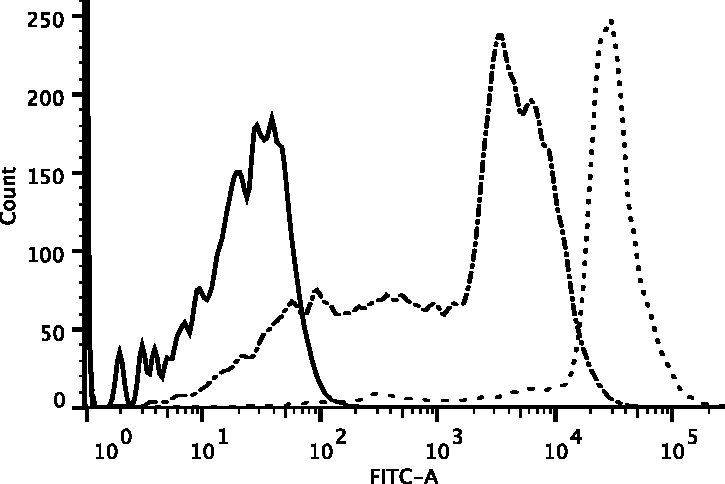
\includegraphics[width=\textwidth]{figs/facs-stable-cell-lines.pdf}
        \captionIntro{Fluorescent intensity of HeLa cell populations
          by flow citometry}%
                     { The multiple populations with differing
                       intensity values were sorted by FACS. The full
                       line represents the intensity profile of HeLa
                       wild type cells, the dash-dot line the mixed
                       population of HeLa cells expressing H2B--EGFP,
                       and the dotted line the homogeneous cell
                       population after sorting.  }
        \label{fig:methods:facs}
      \end{figure}

      Both sample analysis and cell sorting were performed with live cells, the
      first with a BD FACSCanto~II, and the later with a BD FACSAria~II.

  \section{Software used}
    \label{sec:methods:software}
    The European Molecular Biology Open Software Suite (EMBOSS) version 6.4.0
    was used for analysis of codon usage, RNA folding, and reading of
    chromatogram files.

    Image analysis was performed using GNU Octave version \OctaveVersion{},
    and Octave Forge Image, Optim, Statistics, Bioformats, and Signal
    packages, versions \OctaveImageVersion{}, \OctaveOptimVersion{},
    \OctaveStatisticsVersion{}, \OctaveBioformatsVersion{}, and
    \OctaveSignalVersion{} respectively.

    ImageJ, as distributed by the Fiji project, was routinely used
    for microscope image visualization.


  %% To write this chapter we defined a bunch of commands that are
  %% unique to human genome.  We also want to use the same commands
  %% with values for mice genome but the command names.  So we define
  %% the commands locally to this group.  See:
  %% https://tex.stackexchange.com/questions/353002/redefine-existing-commands-outside-preamble
  \chapter{Human Canonical Core Histone Catalogue}
  \begingroup
  \newcommand{\ResultsDir}{results-homo-sapiens}
  \newcommand{\FigsDir}{figs-homo-sapiens}
  \newcommand{\ReferenceDir}{data/reference-homo-sapiens}
  \subinputfrom{histone-catalogue/}{variables}
  \subinputfrom{histone-catalogue/}{manuscript}
  \endgroup

    %% \epigraph{Agora desenmerda-te.}{Portuguese ``saying''}

  \begin{abstract}
    Nucleosomes enable the stable compaction of almost all eukaryotic
    genomes but also require dynamic properties to enable access to
    the packaged DNA sequences.  The stability of core histones within the
    nucleosome should be reflected in their capability for dynamic exchange by
    Fluorescence Recovery After Photobleaching (FRAP).  To assay the
    effect of histone SWI/SNF INdependence (SIN)
    mutants known to destabilise nucleosomes
    \textit{in vitro} and in \species{S. cerevisiae}, we sought to
    apply FRAP to chromatin in mammalian cell lines.  This uncovered a
    number of challenges resulting from cell motility, nuclear movement
    within the cell, and chromatin motion within the nucleus with the
    long time frames required for FRAP of histones.  We were able to
    compensate for the former difficulties by a combination of cell
    biological and computational techniques, but we were unable to
    establish an appropriate approach to compensate for motion of the immobile
    binding sites required for standard FRAP analysis.
    Visualisation using photoactivated tagged histones
    demonstrated the extent of this chromatin motion
    and a further complexity arising from complex
    non-homogenous channelling tagged histone
    during diffusion.  This reveals the
    limitations of FRAP over extremely long time scales, and suggests
    that this technique is unsuitable for quantitative measurement of
    histone dynamics in the mammalian nucleus.
  \end{abstract}

  \section{Introduction}

  Histones are among the most abundant proteins in eukaryotic cells
  and contribute up to half the mass of chromatin \citep{AlbertsMBoC}.
  The core histone types H2A, H2B, H3, and H4
  define the structure and accessibility of the nucleosome
  as the fundamental repeating unit of genome organisation
  around which the DNA is wrapped \citep{Luger1997structure}.
  In addition, the many chemically reactive sidechains of histones
  are post-translationally modified
  as a nexus for signalling and heritable epigenetics \citep{Kouzarides2007}.

  Core histones are delineated as either canonical or variant based on
  their gene location, expression characteristics,
  and functional roles (\tref{tab:typical-histone-differences}).
  Canonical core histones contribute the majority of proteins to
  the bulk structure and generic function of chromatin,
  and are encoded by \TotalCoreGenes{} genes in \NumberOfClusters{}
  clusters named HIST1-HIST\NumberOfClusters{} in the human genome,
  of which \TotalCoreCodingGenes{} are coding genes and \TotalCorePseudoGenes{}
  are pseudogenes (\tref{tab:histone-gene-count}).

  \begin{table}
    \caption{Properties distinguishing canonical and variant core histone proteins.}
    \label{tab:typical-histone-differences}
    \centering
    \begin{tabular}{l l l}
      \toprule
      \null                     & Canonical             & Variants \\
      \midrule
      Expression timing         & Replication dependent & Replication independent \\
      Sequence identity         & High                  & Low \\
      Functional relationships  & Isoforms              & Specialised functions \\
      Transcript stabilisation  & Stem-loop             & poly(A) tail \\
      Gene distribution         & Clusters              & Scattered \\
      \bottomrule
    \end{tabular}
  \end{table}

  \begin{table}
    \caption{Count of human canonical core histone coding genes and pseudogenes
             by histone cluster and type. $\psi$ indicates pseudogenes.}
    \label{tab:histone-gene-count}
    \centering
    \begin{tabular}{l *{5}{r!{+}r<{$\psi$}}}
  \toprule
  \null   & \multicolumn{2}{c}{H2A}  & \multicolumn{2}{c}{H2B}
          & \multicolumn{2}{c}{H3}   & \multicolumn{2}{c}{H4}
          & \multicolumn{2}{c}{Total} \\
  \midrule
  HIST1   & \HTwoACodingInHISTOne{}     & \HTwoAPseudoInHISTOne{}
          & \HTwoBCodingInHISTOne{}     & \HTwoBPseudoInHISTOne{}
          & \HThreeCodingInHISTOne{}    & \HThreePseudoInHISTOne{}
          & \HFourCodingInHISTOne{}     & \HFourPseudoInHISTOne{}
          & \CoreCodingGenesInHISTOne{} & \CorePseudoGenesInHISTOne{} \\
  HIST2   & \HTwoACodingInHISTTwo{}     & \HTwoAPseudoInHISTTwo{}
          & \HTwoBCodingInHISTTwo{}     & \HTwoBPseudoInHISTTwo{}
          & \HThreeCodingInHISTTwo{}    & \HThreePseudoInHISTTwo{}
          & \HFourCodingInHISTTwo{}     & \HFourPseudoInHISTTwo{}
          & \CoreCodingGenesInHISTTwo{} & \CorePseudoGenesInHISTTwo{} \\
  HIST3   & \HTwoACodingInHISTThree{}   & \HTwoAPseudoInHISTThree{}
          & \HTwoBCodingInHISTThree{}   & \HTwoBPseudoInHISTThree{}
          & \HThreeCodingInHISTThree{}  & \HThreePseudoInHISTThree{}
          & \HFourCodingInHISTThree{}   & \HFourPseudoInHISTThree{}
          & \CoreCodingGenesInHISTThree{} & \CorePseudoGenesInHISTThree{} \\
  HIST4   & \HTwoACodingInHISTFour{}    & \HTwoAPseudoInHISTFour{}
          & \HTwoBCodingInHISTFour{}    & \HTwoBPseudoInHISTFour{}
          & \HThreeCodingInHISTFour{}   & \HThreePseudoInHISTFour{}
          & \HFourCodingInHISTFour{}    & \HFourPseudoInHISTFour{}
          & \CoreCodingGenesInHISTFour{} & \CorePseudoGenesInHISTFour{} \\
  \addlinespace
  Total   & \HTwoACodingGenes{}       & \HTwoAPseudoGenes{}
          & \HTwoBCodingGenes{}       & \HTwoBPseudoGenes{}
          & \HThreeCodingGenes{}      & \HThreePseudoGenes{}
          & \HFourCodingGenes{}       & \HFourPseudoGenes{}
          & \TotalCoreCodingGenes{}   & \TotalCorePseudoGenes{} \\
  \bottomrule
\end{tabular}


  \end{table}

  Relationships within the histone family have been described using a variety of terminologies
  reflecting biochemical, functional, and genomic perspectives that are briefly described below
  and summarised in \tref{tab:histone-divisions}.

  \afterpage{
    \captionof{table}{Terminology describing histone variation.}
    \label{tab:histone-divisions}
    \definecolor{shadecolor}{gray}{0.9}
    \begin{shaded}
      \begin{description}
        \item[Allelic variants] \hfill \newline
        Copies of canonical histone type genes,
        possibly with different sequences.
        Not located at same exact chromosomal locus as expected for alleles.
        Not histone variants.
        See also ``isoforms''.

        \item[Canonical core histones]\hfill \newline
        Core histones with properties described in \tref{tab:typical-histone-differences}.
        Contribute the majority of core histones in chromatin.
        Encompasses multiple protein isoforms.
        Complement of variant histones.

        \item[Core histones]\hfill \newline
        Histones that form part of the nucleosome core particle wrapping \SI{147}{\bp} of DNA,
        comprising types H2A, H2B, H3, and H4.
        Encompasses both canonical and variant histones,
        and complements linker histones.

        \item[Heteromorphous variants] \hfill \newline
        Core histone variants with distinct function and localisation
        that are readily separated by gel electrophoresis.

        \item[Homomorphous variants] \hfill \newline
        Canonical core histone subtypes
        requiring high resolution separation methods such as TAU PAGE.
        Synonym for ``subtypes''.

        \item[Families] \hfill \newline
        Synonym for ``histone types''.

        \item[Isoforms] \hfill \newline
        Proteins with high sequence identity and largely equivalent function.
        Functional equivalence has not been demonstrated for canonical histone isoforms.

        \item[Linker histones] \hfill \newline
        Histones binding to linker DNA adjacent to the nucleosome core particle.
        The two linker histone types are H1 and H5. Complement of core histones.

        \item[Non-allelic variants] \hfill \newline
        Synonym for ``variant histones''. See also ``allelic variants''.

        \item[Replacement histones] \hfill \newline
        Synonym for ``variant histones''.
        Named because they can replace canonical core histones assembled in S phase.

        \item[Replication-dependent histones] \hfill \newline
        Synonym for ``canonical core histones''.
        Named because expression occurs primarily in S phase.

        \item[Replication-independent histones] \hfill \newline
        Synonym for ``variant histones''.
        Named because expression is not predominantly in S phase.

        \item[Subtypes] \hfill \newline
        Canonical core histone type isoforms separable by TAU PAGE
        (e.g. H2A.1 and H2A.2).  Despite their naming, there is not necessarily functional evidence
        for differences between them.

        \item[Types] \hfill \newline
        Histone proteins sharing sequence homology
        that participate in specific combinations to define the repeating nucleosome structure.
        The 5 histone types are H1, H2A, H2B, H3, and H4.

        \item[Variant histones] \hfill \newline
        Core histones with properties described in \tref{tab:typical-histone-differences}.
        Contribute a minor proportion of histones in chromatin and perform specialised functions.
        Complement of canonical core histones.

        \item[Wild type histones] \hfill \newline
        Synonym of ``canonical core histones''.
      \end{description}
    \end{shaded}
  }

  \subsection{Biochemical perspective}

    Abundant histone proteins are readily isolated using their
    highly basic chemical character.
    Successive improvements in fractionation ultimately revealed 5 main histone types
    with nomenclature H1, H2A, H2B, H3, and H4 \citep{nomenclature}.
    An additional H1-related histone H5 is recognised in avian erythrocytes \citep{HFive-review}.

    The demonstration of the nucleosome as the fundamental
    repeating unit of chromatin \citep{Kornberg1974}
    showed that H2A, H2B, H3, and H4 associate as an octamer of two copies each within the
    nucleosome core particle. These four histones are referred to as core histones.
    In contrast, H1 associates with the linker DNA between nucleosome core particles
    and is referred to as a linker histone.
    The somatic H1 isoforms and its tissue-specific
    variants are described elsewhere \citep{HarshmanFreitas2013}.

    Arginine and lysine content was used as an early distinction between the histones \citep{ElginWeintraub1975}.
    The H1 linker histone has a low arginine/lysine ratio of
    \FPround{\result}{\LinkerArgLysRatio}{2} \result{}
    and became known as lysine-rich
    whereas the 4 core histones are arginine-rich
    with high arginine/lysine ratios of
    \FPround{\result}{\HTwoAArgLysRatio}{2} \result{} in H2A,
    \FPround{\result}{\HTwoBArgLysRatio}{2} \result{} in H2B,
    \FPround{\result}{\HThreeArgLysRatio}{2} \result{} in H3,
    and \FPround{\result}{\HFourArgLysRatio}{2} \result{} in H4 type isoforms.
    Nevertheless, the core histones contain many lysines particularly in their N-terminal tails.

    Separating histones by polyacrylamide gel electrophoresis (PAGE)
    using the strongly anionic detergent sodium dodecyl sulphate and neutral buffers (SDS PAGE)
    gives single bands for each histone type \citep{ShechterHake2007}.
    However, PAGE with non-ionic detergent Triton X--100 and urea as denaturants
    in acid buffers (TAU or AUT PAGE) allows the separation
    of histone types into multiple bands
    due to post-translational modifications and differences at specific amino acids
    in the polypeptides \citep{Zweidler1977}.
    These TAU PAGE separations gave rise to subtype designations
    H2A.1, H2A.2, H3.1, H3.2, and H3.3.

  \subsection{Functional perspective}

    Canonical core histone expression
    is significantly elevated during S~phase to provide chromatin packaging
    for DNA duplicated during replication \citep{WuBonner1981}.
    This led to their description as ``replication dependent'',
    although a supply of canonical histones is inevitably required
    to partner variants throughout the cell cycle.
    Metazoan canonical core histone genes are distinctive
    because they lack introns and give rise to non-polyadenylated protein coding transcripts.
    Turnover is independently regulated via a highly
    conserved 3' stem-loop (\tref{tab:typical-histone-differences}).

    In contrast, variant histones such as H2A.Z, TH2B, H3.3, and CENP-A have
    reduced sequence identity and lower abundance \citep{TalbertHenikoff2010}.
    They play functionally specific roles and are mostly expressed outside S~phase,
    so are described as ``replication independent''.
    Since histone variants are interpreted as taking the place
    of equivalent canonical core histone types,
    they are also referred to as ``replacement'' histones.

  \subsection{Genomic perspective}

    Canonical core histone genes are found in \NumberOfClusters{} clusters.
    The multiple gene copies in these clustered arrays are
    sometimes confusingly referred to as ``allelic''
    and the resulting combined protein isoforms are often considered to be ``wild type''
    although both genes and protein products display
    variation in primary sequence and relative abundance,
    and their functional equivalence has not been tested.
    In contrast, almost all variant histones are encoded by single genes dispersed in the genome
    with typical properties including introns, alternative splicing,
    and polyadenylated transcripts (\tref{tab:typical-histone-differences}).

  \subsection{Curation of canonical core histone diversity}

    Despite the importance of histones for chromatin organisation and extensive interest
    in their role in epigenetics and regulation, the systematic
    curation and classification of human histone
    gene and protein sequences has not been revisited
    since the landmark 2002 survey by \citet{Marzluff02}.
    The canonical core histone catalogue has since accumulated
    \TotalChangesSinceReference{}~differences (\tref{tab:difference-from-Marzluff02})
    from that survey due to rich annotations continuing to propagate
    into reference sequence databases.

    In this manuscript we provide a comprehensive catalogue
    of canonical core histone genes, encoded proteins, and pseudogenes
    based on reference genome annotations.
    This reveals a surprising and seldom recognised variation in encoded histone proteins
    that exceeds commonly used subtype designations
    but whose functional implications have not been investigated.

    Since curation and annotation are dynamic and evolving, we have
    implemented the manuscript so that it can be regenerated from the
    most current data in the NCBI RefSeq database in order to maintain
    its value as a reference source in an accessible format.  All
    figures and tables were automatically generated using NCBI RefSeq
    data from \printdate{\SequencesDate{}}.  In addition,
    automatically generated values in the text are displayed with a
    light grey background.  This manuscript generation process has
    remained stable in our laboratory for several years and represents
    an example of ``reproducible research'' \citep{Claerbout2000} that
    provides a novel model for curating relatively stable gene
    families.

  \chapter{Materials and Methods}
\label{ch:methods}

  %% \epigraph{As palavras que nunca te direi.}{Translation of ``Message in a bottle''}
  %% \epigraph{The devil is in the details.}

  All chemicals used were purchased from Sigma unless otherwise stated. All
  solutions were prepared according to \tref{tab:methods:solutions} with Milli-Q
  purified water, and autoclaved prior to use when appropriate.

  %% FIXME Depending on what border and font size we use at the end,
  %%       this may fit in a single page and then we can drop the use
  %%       of longtable and have a regular table without need for
  %%       afterpage.

  %% longtable does not float so it would appear right here halfway
  %% the very first page of the methods chapter.  We use afterpage to
  %% delay it to the strat of the next page.
  \afterpage{
    %% The way we calculate the columns width (with eqparbox), doesn't work
    %% with memoir's ctabular so we are using longtable instead.
    %%
    %% An alternative method to make this list is with description environment
    %%
    %% \begin{description}
    %%   \item[Freezing media] \hfill \\
    %%     91\% FCS;
    %%     10\% DMSO
    %%   \item[Growth medium (HeLa)] \hfill \\
    %%     87\% DMEM;
    %%     10\% FCS;
    %%     1\% NEAA;
    %%     ...
    %% \end{description}
    \begin{longtable}{>{\bfseries}\SolutionNameCol
        p{\dimexpr(\textwidth-\eqboxwidth{SolutionNameBox}-4\tabcolsep)}}
      \captionIntro{Commonly used buffers and media}{}
      \label{tab:methods:solutions}
      \endfirsthead
      \endhead
      \toprule
      Name & Recipe\\
      \midrule
      2YT broth               & \SI{16}{\g\per\l} tryptone;
      \SI{10}{\g\per\l} yeast extract;
      \SI{5}{\g\per\l}  NaCl.\\

      DMEM                    & \SI{4.5}{\g\per\l}   glucose;
      \SI{110}{\mg\per\l}  L-glutamine;
      \SI{584}{\ug\per\l}  sodium pyruvate;
      \SI{15.9}{\mg\per\l} phenol red.\\

      DNA loading buffer (\SI{10}{\X}) & \pcent{25} Ficoll ($w/v$);
      \SI{100}{\mM}      Tris--HCl pH=\num{7.4};
      \SI{100}{\mM}      EDTA.\\

      FACS buffer             & \pcent{96} PBS ($v/v$);                   % 480.5 mL
      \SI{2}{\mM} EDTA;                         % 2 mL
      \SI{25}{\mM} HEPES buffer pH=\num{7.0};   % 12.5 mL
      \pcent{1} FCS ($v/v$).\\                  % 5 mL

      Freezing media          & \pcent{90} FCS ($v/v$);
      \pcent{10} DMSO ($v/v$).\\

      Growth medium (HeLa, HEp2) & \pcent{89}         DMEM ($v/v$);   % 500ml
      \pcent{9}             FCS ($v/v$);    % 50ml
      \SI{1}{\X}            NEAA solution;  % 5.5mL
      \SI{50}{units\per\ml} penicillin;     % 5.5mL (Pen/Strep solution)
      \SI{50}{\ug\per\ml}   streptomycin.\\ % 5.5mL (Pen/Strep solution)

      Growth medium (horse)   & \pcent{81}            DMEM ($v/v$);   % 500ml
      \pcent{16}            FCS ($v/v$);    % 100ml
      \SI{2}{\X}            NEAA solution;  %  12mL
      \SI{50}{units\per\ml} penicillin;     % 5.5mL (Pen/Strep solution)
      \SI{50}{\ug\per\ml}   streptomycin.\\ % 5.5mL (Pen/Strep solution)

      LB agar                 & \SI{20}{\g\per\l}  LB broth powder;
      \SI{7.5}{\g\per\l} agar.\\

      LB broth                & \SI{20}{\g\per\l} LB broth powder.\\

      Ponceau S solution      & \pcent{5} Ponceau S ($w/v$);
      \pcent{5} Acetic acid ($v/v$).\\

      Running buffer          & \SI{1}{\X}  TG;
      \pcent{0.1} SDS ($w/v$).\\

      SSC (Saline Sodim Citrate) & \SI{150}{\mM} NaCl;
      \SI{15}{\mM}     trisodium citrate.\\

      TAE (Tris Acetate EDTA) & \SI{40}{\mM} Tris;
      \SI{20}{\mM} acetic acid;
      \SI{1}{\mM}  EDTA.\\

      TBE (Tris Borate EDTA)  & \SI{89}{\mM} Tris;
      \SI{89}{\mM} boric acid;
      \SI{2}{\mM}  EDTA.\\

      TBS (Tris Buffered Saline)  & \SI{50}{\mM} Tris--HCl pH=\num{7.5};
      \SI{100}{\mM}    NaCl.\\

      PBS-T (TBS-Tween)       & \pcent{99.95} PBS ($v/v$);
      \pcent{0.05}  Tween 20 ($v/v$).\\

      TG (Tris Glycine)       & \SI{25}{\mM}  Tris;
      \SI{192}{\mM} glycine.\\

      Transfer buffer         & \SI{1}{\X} TG;
      \pcent{15} methanol ($v/v$).\\
      \bottomrule
    \end{longtable}
  }

  Restriction enzymes, T4 DNA ligase, other DNA modifying enzymes, and DNA
  ladders were obtained from New England BioLabs.
  Protein ladders were obtained from Invitrogen.

  For use in tissue culture, FCS and DMEM (without phenol red and L-glutamine)
  were obtained from Lonza.  DMEM (supplemented with glucose, sodium pyruvate,
  L-glutamine and phenol red), Non-Essential Amino Acid (NEAA) solution, and
  PBS (without Ca$^{2+}$ and Mg$^{2+}$) were obtained from Sigma.
  Penicillin--Streptomycin
  solution and Trypsin--EDTA were obtained from Gibco.

  \section{DNA methods}
    \subsection{Bacterial cultures}
      \species{E.~coli} cultures were prepared with either LB broth or agar
      at \dc{37}. For antibiotic selection, ampicillin, kanamycin, and
      chloramphenicol, were used at concentrations of 100, 30,
      and \SI{34}{\mg\per\l} respectively.

    \subsection{Preparation of competent bacteria}
      Competent \species{E.~coli} cells were prepared from a culture of
      Invitrogen's One Shot TOP10 Chemically Competent \species{E.~coli}. LB
      cultures of \SI{1}{\l} were grown at \dc{37} until an OD$_{\SI{600}{\nm}}$
      of \numrange{0.4}{0.5}.  Subsequent steps were carried at \dc{4} with
      previously chilled equipment and solutions.

      Cultures were centrifuged at \SI{6000}{\gn} for 10 minutes, the
      pellet was resuspended in \SI{500}{\ml} of \SI{0.1}{\mM} CaCl$_2$, and
      incubated on ice for 30 minutes. The suspensions were centrifuged
      again at \SI{6000}{\gn} for 10 minutes,
      and the resulting pellet resuspended in
      \SI{100}{\ml} of CaCl$_2$ with \pcent{15} glycerol. Aliquots of
      competent cells were prepared and stored at \dc{-80}.

      Transformation efficiencies were measured after preparation of each
      batch and discarded if less than \SI{1d6}{\cfu\per\mg} of plasmid was
      obtained. Absence of antibiotic-resistant contaminations was assessed
      by streaking the cells on selective plates.

    \subsection{Transformation of competent cells}
      Competent cells were thawed on ice and split into aliquots of
      \SI{50}{\ul} to pre-chilled \SI{2}{\ml} tubes where
      \SI{1}{\ul} of \SI{\approx 100}{\ng\per\ul} DNA
      was added. Cells were incubated on ice for 30 minutes, followed by a
      60 seconds heat-shock at \dc{42}, and 5 more minutes on ice.
      \SI{300}{\ul} of non-selective LB was added to each tube and the
      cultures incubated at \dc{37} with vigorous shaking for 45 minutes.
      Samples from the cultures were then plated onto the appropriate
      antibiotic containing agar plates, and incubated overnight at \dc{37}.

      For concentrations of plasmid DNA higher than \SI{500}{\ng\per\ul}, only
      \SI{0.3}{\ul} of DNA was used, and both the initial and final incubation
      steps were shorted to 10 minutes.

    \subsection{Plasmid DNA preparation}
      Plasmid DNA was prepared with QIAprep Spin Miniprep,
      QIAGEN Plasmid \textit{Plus} Midi, QIAquick Gel Extraction, and QIAquick
      PCR purification kits from QIAGEN
      according the manufacturer's instructions.
      Once prepared, DNA was stored at \dc{-20}.
      DNA concentrations were measured
      with a spectrophotometer (NanoDrop 2000c spectrophotometer from
      Thermo Scientific).

    \subsection{Ethanol precipitation}
      \label{sec:ethanol-precipitation}
      The DNA solution was mixed with \num{2.5} volumes of \pcent{100} ethanol
      and \num{1/10} volumes of Sodium Acetate (\SI{3}{\Molar}, pH=\num{5.2}),
      and incubated at \dc{4} for 15 minutes. When DNA concentrations were below
      \SI{50}{\ng\per\ul}, incubations were performed overnight.
      DNA solution was then centrifuged at
      \SI{18000}{\gn} for 30 minutes at \dc{4} and the supernatant discarded.
      The pellet was left to dry until all traces of solvent evaporated.
      DNA pellet
      was resuspended in the desired solvent:
      H$_2$O when being used for transfection,
      EB~buffer from QIAGEN in all other cases.

    \subsection{Agarose gel electrophoresis}
      Agarose gels with concentrations ranging from \SIrange{0.6}{2.0}{\percent}
      were prepared with TAE buffer, and supplemented with ethidium bromide.
      DNA samples were loaded into the gel with DNA loading buffer and a
      choice of loading dyes between bromophenol blue, cresol red, orange G, or
      xylene cyanol.  In each case, the appropriate dye was chosen
      to avoid shadowing of the DNA bands. Electrophoresis was
      performed in Owl EasyCast electrophoresis chambers with
      \SI{1}{\X}~TAE buffer at
      \SIrange{80}{120}{\volt} until the required separation was achieved.
      Gels were visualized using a
      Alpha Innotech ChemiImager 5500 UV transilluminator.

    \subsection{DNA sequencing and oligonucleotide preparation}
      DNA sequencing was performed by LGC Genomics after cloning for sequence
      confirmation and avoiding unexpected mutations.

      Oligonucleotides were ordered from Eurofins MWG operon in lyophilized
      format, dissolved in H$_2$O to a \SI{100}{\micro\Molar} concentration,
      and stored at \dc{-20}. A list of all designed oligonucleotides is
      shown in \Aref{app:primers}.

    \subsection{Polymerase Chain Reaction}
      Different types of PCR experiments were performed for different purposes
      using a selection of DNA polymerases (\tref{tab:pcr-settings}).
      Taq polymerase with ThermoPol
      buffer was obtained from New England Biolabs.
      KOD Hot Start DNA polymerase with Mg$^{2+}$
      free buffer was obtained from Novagen. PCRs were performed on a
      Mastercycler epgradient thermocycler from Eppendorf.

      Use of different DNA polymerases was based on their cost-benefit for
      each application. For example, screening clones requires a large number
      of reactions in tandem and the introduction of small mutations
      is of no consequence. For these two reasons, the much cheaper Taq DNA
      polymerase was used for screening despite its relatively low fidelity and
      amplification rates. However, in PCR mutagenesis the whole plasmid
      is synthesised anew and we have no reasonable method to verify
      the entire plasmid
      sequence. As a result, KOD DNA polymerase was used for PCR mutagenesis.

      \begin{sidewaystable}
        \centering
        \captionIntro{PCR mixtures and conditions used}
          {
            Since each reaction was unique, with different pair of primers
            and template DNA, the optimal salt concentrations, temperature
            of the annealing step, and time of extension step actually used were
            sometimes different. Listed values correspond to the most common
            usage.
          }
        \label{tab:pcr-settings}

        \newcolumntype{W}{r<{\si{\second}}}
        \newcolumntype{T}{l<{\si{\degreeCelsius}}}

        \begin{tabular}{l W@{ at }T W@{ at }T W@{ at }T W@{ at }T W@{ at }T}
          \toprule
          \null                        & \multicolumn{4}{c}{cloning} & \crows{colony} & \crows{mutagenesis} & \crows{screening} \\
                                                \cmidrule(r){2-5}
          \null                        & \crows{genomic} & \crows{plasmid} \\
          \midrule
          Template (\si{\ng})          & \crows{1000}      & \crows{50}        & \crows{n/a}       & \crows{750}       & \crows{50}        \\
          DMSO (\si{\ul})              & \crows{---}       & \crows{---}       & \crows{1}         & \crows{---}       & \crows{1}         \\
          Buffer (\si{\X})             & \crows{1}         & \crows{1}         & \crows{1}         & \crows{1}         & \crows{1}         \\
          MgSO$_4$ (\si{\nmol})        & \crows{1.5}       & \crows{1.5}       & \crows{---}       & \crows{1.5}       & \crows{---}       \\
          dNTPs (\si{\mM} each)        & \crows{0.2}       & \crows{0.2}       & \crows{0.2}       & \crows{0.2}       & \crows{0.2}       \\
          Primer (forward) (\si{\uM})  & \crows{2}         & \crows{2}         & \crows{2}         & \crows{0.4}       & \crows{2}         \\
          Primer (reverse) (\si{\uM})  & \crows{2}         & \crows{2}         & \crows{2}         & \crows{0.4}       & \crows{2}         \\
          DNA polymerase (\si{U})      & \crows{0.5 (KOD)} & \crows{0.5 (KOD)} & \crows{2.5 (Taq)} & \crows{0.5 (KOD)} & \crows{2.5 (Taq)} \\
          \addlinespace
          Total volume (\si{\ul})      & \crows{25}        & \crows{25}        & \crows{25}        & \crows{25}        & \crows{25}        \\
          \addlinespace
          \midrule
          \addlinespace
          Initialization                & 120 & 94    & 120 & 94    & 180 & 94    & 120 & 94    & 120 & 94 \\
          Denaturation                  &  30 & 94    &  30 & 94    &  15 & 94    &  30 & 94    &  15 & 94 \\
          Annealing                     &  20 & 58    &  20 & 58    &  15 & 58    &  20 & 58    &  15 & 62 \\
          Extension (per \si{\kilo\bp}) &  30 & 68    &  20 & 72    &  60 & 72    &  30 & 68    &  60 & 72 \\
          Final extension               & 300 & 62    & 300 & 72    & 300 & 72    & 300 & 68    & 300 & 72 \\
          Final hold       & \crows{\dc{4}}      & \crows{\dc{4}}      & \crows{\dc{4}}      & \crows{\dc{4}}      & \crows{\dc{4}} \\
          Number of cycles & \crows{\SI{30}{\X}} & \crows{\SI{30}{\X}} & \crows{\SI{30}{\X}} & \crows{\SI{15}{\X}} & \crows{\SI{20}{\X}} \\
          \bottomrule
        \end{tabular}
      \end{sidewaystable}

      \subsubsection{Colony PCR}
        When screening multiple clones after transformation and a set of
        appropriate primers was available, PCRs were carried out directly on
        the bacteria colonies by adding them directly to the reaction mixture
        (\tref{tab:pcr-settings}). Bacteria from individual colonies were
        used to simultaneously perform a PCR and start a small culture.
        Plasmid purification was performed on cultures whose sample was
        confirmed to be the desired product by a positive PCR result.

      \subsubsection{Gene cloning}
        PCRs were used to clone and subclone genes from genomic DNA and
        plasmids, into different vectors. Primers were usually
        extended to introduce restriction sites and create DNA linkers.
        Additional extensions were added to the
        5' end of primers to account for the minimum
        required \si{\bp} around the restriction sites
        \citep{neb_catalogue_2011} \todo{correct format}.

      \subsubsection{Mutagenesis}
        PCR mutagenesis
        \footnote{
          In PCR mutagenesis, since the newly synthesized strands will
          be linear and cannot be used as template, the amplification
          is linear rather than exponential. Because of this, the name
          PCR mutagenesis is misleading. There is in fact no chain reaction.
        }
        was used to insert or correct mutations in plasmids.
        Where possible, the selected codon used for mutation was the one
        with highest frequency in the organism used for expression
        in accordance with the
        codon usage database \citep{codon_usage}. After amplification,
        \SI{1.5}{\ul} of the restriction enzyme DpnI
        \footnote{
          Because DpnI activity is blocked by DNA methylation, it will
          only digest the template DNA which was synthesized in bacteria,
          leaving the newly \textit{in vitro} synthesized DNA intact.
        }
        was added directly to the PCR mixture, and incubated overnight at
        \dc{37}. \SI{1}{\ul} of reaction product
        was used for transformation and individual
        clones screened by sequencing.

      \subsubsection{Screening plasmid}
        PCRs were frequently used to screen plasmids for DNA sequences
        in the absence of opportune restriction sites or even plasmid maps.

    \subsection{Plasmid construction}

      \paragraph{pBOS--H2B--EGFP D25G V118I}
      Plasmid was provided by Prof.\@ Kevin Sullivan (NUIG) from
      previous work \citep{KevinH2BGFP}.  DNA sequencing identified
      gene \gene{HIST1H2BJ} as the closest human H2B in RefSeq but
      with missense mutations D25G and V118I.

      \paragraph{pBOS--H2B--EGFP}
      The D25G and V118I mutations in pBOS--H2B--EGFP were corrected
      by PCR mutagenesis using primers AFG114 and AFG115, and AFG112
      and AFG113 respectively.  The resulting product encodes the
      \gene{HIST1H2BJ} RefSeq gene.

      \paragraph{pBOS--EGFP}
      The pBOS--H2B--EGFP was digested with KpnI and BamHI and the
      band corresponding to the linearised vector, without the H2B
      sequence, was purified by gel extraction.  This linearised vector
      was used as backbone vector for the other pBOS constructed
      plasmids.

      \paragraph{pBOS--H2A--EGFP}
      The \gene{HIST1H2AB} gene sequence was amplified from HeLa
      genomic DNA with primers AFG116 and AFG118, the PCR product
      digested with KpnI and BamHI, and then ligated into the
      pBOS--EGFP vector.  The \gene{HIST1H2AB} was chosen because it
      encodes the same protein as the H2A used in previous work
      \citep{flaus2004sin}.  The only other available alternative
      that encoded the same protein was \gene{HIST1H2AE}.
      However, the \gene{HIST1H2AE} sequence has a lower codon
      adaptation index and more stable predicted 5' mRNA secondary structure.

      \paragraph{pBOS--H2AX--EGFP}
      The \gene{H2AFX} gene sequence was amplified from HeLa genomic
      DNA with primers AFG130 and AFG131.  The same strategy used in
      the cloning of pBOS--H2A--EGFP was used.  An accidental
      frameshift mutation near the stop codon was posteriorly fixed by
      PCR mutagenesis using primers AFG400 and AFG401.

      \paragraph{pBOS--H2AX--EGFP S139 mutants}
      For H2AX S139 mutations, the \gene{H2AFX} gene sequence was
      amplified from HeLa genomic DNA in the same reaction that the
      mutations were introduced since their location is close to the
      sequence 3' end.  Primers AFG132, AFG133, and AFG134, were used
      with AFG130 to introduce H2AX mutations S139A, S139D, and S139E
      respectively.  The mutation to alanine blocks phosphorylation of
      S139, while mutation to aspartic and glutamic acid mimic
      phosphorylation of S139.  The same strategy used in the cloning
      of pBOS--H2AX--EGFP was used, including the correction of a
      frameshift mutation with AFG400 and AFG401.

      %% Note: not gene sequence so we don't talk about the gene and
      %%       therefore not in italic (and we don't use \gene)
      \paragraph{pBOS--H2A.Z--EGFP}
      Due to the presence of introns in the \gene{H2AFZ} gene
      sequence, the transcript sequence was amplified from HeLa cDNA
      provided by Dr.\@ Nadine Quinn \citep{NadineThesis}.  The
      amplification was performed with primers AFG121 and AFG122, and
      the product cloned into the pBOS--EGFP with the same strategy
      used for pBOS--H2A--EGFP.

      \paragraph{pBOS--H3--EYFP.MC--N1}
      Plasmid was provided by Prof.\@ Kevin Sullivan (NUIG).  DNA
      sequencing identified the H3 sequence as the human RefSeq
      \gene{HIST1H3B} gene, encoding H3.1 from histone cluster 1.

      \paragraph{pBOS--H3--EYFP T45A and T45E}
      Mutations to H3 T45 were inserted into pBOS--H3--EYFP.MC--N1 by
      PCR mutagenesis. The primers AFG151 and AFG152 were used
      to generate the
      T45E mutation, and AFG153 and AFG154 for T45A.

      \paragraph{pBOS--H4--ECFP.M--N1}
      Plasmid was provided by Prof.\@ Kevin Sullivan (NUIG).  DNA
      sequencing identified the H4 sequence as the human RefSeq
      \gene{HIST1H4J} or \gene{HIST1H4K}, both of which have the same
      genomic sequence.

      \paragraph{pBOS--H4--ECFP R45H}
      The H4 R45H mutation was inserted into pBOS--H4--ECFP.M--N1 by
      PCR mutagenesis using the primers AFG124 and AFG125. The codon
      \texttt{CAC} was selected for the histidine amino acid due to
      its higher codon usage in the human genome \citep{codon_usage}.

      \paragraph{pBOS--H4--EYFP}
      The plasmid pBOS--H3--EYFP.MC--N1 was digested with the
      restriction enzymes BamHI and NotI to extract the EYFP sequence
      which was purified by agarose gel extraction.  The pBOS--H4
      sequence was prepared in the same manner from
      pBOS--H4--ECFP.M--N1.  The two fragments were ligated to
      construct pBOS-H4-EYFP.

      \paragraph{pBOS--H4--EYFP R45H}
      The same strategy used for the cloning of wild type
      pBOS--H4--EYFP was used for the R45H mutant using
      pBOS--H4--ECFP R45H.

      \paragraph{PA-GFP}
      The PA-GFP sequence used as an insert for other plamids was
      amplified from pPA-GFP--N1 with primers AFG478 and AFG479.  The
      amplicon was purified by agarose gel extraction, digested with
      NotI and BamHI, and then cleaned by PCR purification.  The
      pPA-GFP--N1 plasmid was a kind gift from Chelly van Vuuren
      (NUIG).

      \paragraph{pBOS--H2B--PA-GFP}
      The plasmid pBOS--H2B--EGFP was digested with NotI and BamHI
      which removed the EGFP sequence.  The vector was purified by
      agarose gel extraction and ligated with the PA-GFP insert.  This
      strategy introduced a proline to arginine mutation in the linker
      sequence between H2B and PAGFP when compared to the linker
      sequence between H2B and EGFP.
      %% This mutation in the H2B linker (DPPVAT to DPRVAT) was not on
      %% purpose but wasn't an accident either.  We knew about it and
      %% could have easily avoid it but would cost us one extra primer
      %% and it shouldn't be making a difference.

      \paragraph{pBOS--H3--PA-GFP}
      The plasmid pBOS--H3--EYFP.MC--N1 was digested with NotI and
      BamHI which removed the EYFP sequence.  The vector was purified
      by agarose gel extraction and ligated with the PA-GFP insert.
      %% Unlike the H2B--PA-GFP plasmid, this did not introduce any
      %% mutation in the linker sequence.

      \paragraph{mCherry--\textalpha--tubulin}
      Plasmid was a kind gift from Chelly van Vuuren (NUIG).

      %% I'm actually not sure if Kevin gave me the pMH3.2--614 or the
      %% pCA-TAG plasmid. I did not have any plasmid map or sequence, only
      %% the very small Figure 5 of his paper PMID:9024683
      %% I couldn't even use any standard sequencing primer and by the time
      %% we cloned our genes there, we had already decided to kill the project
      %% so we never got to actually try these in human cells.
      \paragraph{pMH3.2--614}
      The plasmid includes a mouse replication dependent histone H3.2
      gene with upstream and downstream regulatory elements
      \citep{pMH3-plasmid}.  It was provided by Prof.\@ Kevin
      Sullivan.  Due to the absence of convenient restriction sites in
      the plasmid, insertion of alternative histone gene sequence was
      performed by blunt-end ligation of PCR products.  pMH3.2--614
      was amplified with primers AFG417 and AFG418 which amplified the
      vector backbone, including the upstream and downstream
      regulatory elements but ignored the H3.2 coding sequence.  The
      amplified sequence was purified by agarose gel extraction to be
      used in the cloning of pM-H2B--EGFP and pM-H3--EYFP.

      \paragraph{pM-H2B--EGFP and pMH3--EYFP}
      The H2B--EGFP insert sequence was generated by PCR amplification
      with primers AFG419 and AFG420, purified by agarose gel
      extraction, and ligated into the pMH3.2--614 vector.  The
      primers for the insert, AFG419 and AFG420, were phosphorylated
      by T4~PNK prior to PCR since T4~PNK is more efficient on single
      stranded DNA.
      The same strategy was used for the cloning of pMH3--EYFP using
      primers AFG424 and AFG420.

  \section{Protein methods}
    \subsection{Phenol:chloroform extraction}
      \label{sec:phenol-extraction}
      To extract proteins, an equal volume of phenol:chloroform was
      added and the mixture centrifuged at \SI{6000}{\gn} for 15 minutes.
      The top aqueous phase (chloroform) was pipetted to a new tube and
      the process repeated a total of 3 times.

    \subsection{Western blotting}
      \subsubsection{Protein concentration determination}
        Concentration of protein was measured with Bradford reagent.
        \SI{2}{\ul} of the sample after sonication (\Sref{sec:cell-extract})
        was mixed with \SI{48}{\ul} of H$_2$O and \SI{50}{\ul} of NaOH and
        incubated at \dc{65} for 8 minutes before adding \SI{900}{\ul} of
        Bradford reagent from Pierce. The mixture was transferred to plastic
        cuvettes and the absorbance at \SI{595}{\nm} measured in a Shimadzu
        spectrophotometer. The values obtained were interpolated from a
        standard curve prepared using known concentrations of BSA.

      \subsubsection{SDS--PAGE}
        Resolving and stacking SDS--PAGE gels of \SIrange{15}{5}{\percent}
        respectively, both with a cross-linking ratio of \num{37.5}:1 as
        described in \citet{harlow_electrophoresis_1988} were used. The
        resolving gel was poured directly after addition
        of TEMED and it was covered with a layer of isopropanol during polymerisation
        to ensure a sharp interface between the resolving and stacking layers.
        Protein samples and markers were boiled at \dc{99} for 3 minutes and each
        was loaded twice, with volumes for \SI{3.3}{\ug} and \SI{16.5}{\ug} of
        protein. Gels ran at \SI{180}{\volt} for 1 hour in \SI{1}{\X} TG buffer.

      \subsubsection{Protein transfer}
        Protein transfer occurred through the wet transfer system. The
        SDS-PAGE gel was placed onto pre-cut nitrocellulose transfer membrane
        previously soaked in transfer buffer. It was then set between a pair
        of extra thick blotting paper and cushions before being placed inside
        a transfer apparatus. The transfer ran at \dc{4} for 60
        minutes at \SI{100}{\volt}.

      \subsubsection{Probing of blot with antibody}
        Blocking of the membrane was performed with \SI{10}{\percent}
        non-fat dry milk (Marvel) in \SI{1}{\X} TBS-T buffer
        at room temperature for 30 minutes. Blocking was followed by
        primary antibody incubation which occurred in \SI{5}{\percent} non-fat
        dry milk in \SI{1}{\X} TBS-T overnight at \dc{4}. Concentrations of
        antibody used were 1:500 and 1:20000 for anti-GFP (catalogue
        number 11~814~460~001 from Roche) and anti-H3 (code ab1791 from
        abcam). The membrane was then washed with \SI{1}{\X} TBS-T for
        15 minutes 3 times before secondary antibody incubation
        in \SI{5}{\percent} non-fat dry milk with \SI{1}{\X} TBS-T for
        1 hour. The membrane was washed once more in the same
        conditions as before for the detection. All blocking, antibody
        incubation and washing steps occurred on a rocker.

        Detection was performed using the SuperSignal West Pico Chemiluminescent
        Substrate from Pierce, adding 1:1 of the solutions and allowing it to incubate
        with the membrane for 5 minutes. The membrane was exposed to x-ray films for
        10, 60, 5, 180 and 1800 seconds which were then developed.


  \section{Cell methods}
    \subsection{Cell culture}
      HeLa (ATCC CCL-2) and HEp-2 cells were supplied by
      Dr.\@ Agnieszka Kaczmarczyk \citep{AgaThesis}
      and Dr.\@ Volker Döring \citep{VolkerThesis} respectively.
      Primary horse fibrolasts were a gift from Prof.~Elena Giulotto from the
      University of Pavia, Department of Genetics and Microbiology.

      All cell lines were maintained at \dc{37}
      and \pcent{5} CO$_2$ in \SI{10}{\cm}
      diameter plates with \SI{10}{\ml} of their respective growth
      medium \trefp{tab:methods:solutions}.
      Once cells reached a confluence of \SIrange{80}{90}{\percent},
      they were trypsinised and split.  First they were washed with
      Dulbecco's Phosphate Buffered Saline (DPBS) solution and then
      incubated at \dc{37} for 5 minutes in \SI{2}{\ml} of
      trypsin--EDTA.  Finally, they were diluted 1:10 in fresh media
      and transferred to a new plate.

    \subsection{Cell stock storage}
      For long-term storage of HeLa cell lines, they were grown until
      they reached a confluence of \SIrange{80}{90}{\percent} and then
      trypsinised. A volume of Freezing Media was added, equal
      to the volume of trypsin--EDTA, and \SI{2}{\ml} aliquots of
      cells transferred to cryotubes. Tubes were immediately wrapped in
      cotton and placed at \dc{-80}.

    \subsection{Whole cell extract}
      \label{sec:cell-extract}
      To obtain whole cell extracts, HeLa cells were trypsinized as usual. Growth
      medium added and the suspension was centrifuged at \SI{900}{\gn}
      for 10 minutes.
      Subsequent steps were carried out at \dc{4} and with previously
      chilled reagents. The supernatant was discarded and the pellet
      resuspended in \SI{500}{\ul} of chilled PBS before being
      sonicated 3 times at \pcent{40} amplitude for 10 seconds. Avoiding the
      formation of foam at the top, \SI{300}{\ul} of suspension was transferred
      from the bottom of the tube to a new \SI{1.5}{\ml} tube
      and mixed with an equal
      volume of Laemmli buffer before being stored at \dc{-80}.
      \SI{2}{\ul} from the suspension was also transferred to a new tube
      for determination of protein concentration by Bradforf protein assay.

    \subsection{Genomic DNA extraction}
      To extract genomic DNA from HeLa cells, they were trypsinised and
      growth medium was added before counting with an hemocytometer.
      Cells were centrifuged at \SI{1500}{\gn} for 10 minutes at \dc{4}, the
      supernatant was discarded
      and the pellet resuspended in TE buffer to achieve
      a desired concentration of \SI{4e7}{cells\per\ml}. 9 volumes of
      genomic lysis buffer was added
      and the mixture was incubated at \dc{37} for
      90 minutes. Proteinase K was then added to a final concentration of
      \SI{100}{\ug\per\ml} and the mixture was
      incubated at \dc{50} for 3 hours and
      swirled every 20 minutes. DNA was then extracted by
      phenol:chloroform (\Sref{sec:phenol-extraction}) and purified by ethanol
      precipitation (\Sref{sec:ethanol-precipitation}).

    \subsection{Viable cells count}
      \label{sec:methods:trypan-blue}
      Trypan blue was used to assess the number of viable cells.
      After trypsinisation, cells were diluted in growth media,
      to a final concentration of \SI{2e5}{cells\per\ml}.
      To \SI{0.5}{\ml} of the cell suspension, \SI{0.1}{\ml} of \pcent{0.4}
      Trypan Blue Stain was added and the mixture left for 5 minutes
      at room temperature before counting
      the cells in an hemocytometer and making a distinction between
      stained (non-viable) and non-stained (viable) cells.

    \subsection{Kill curve}
      \label{sec:methods:kill-curve}
      Cells were trypsinised and plated at \pcent{25} confluence on
      a 24-well plate. After 24 hours, medium was replaced using different
      concentrations of the antibiotic per well, 3 replicas for each.
      After 3 days, medium was replenished
      with the same antibiotic concentrations. After 4 days, a total of
      one week after addition of antibiotics, cells were trypsinised and a count
      of viable cells was performed with
      Trypan Blue (\Sref{sec:methods:trypan-blue}).

      The highest concentration tested with no viable cells in all
      replicas after 7 days was used for selection of transfected
      cells when establishing stable cell lines.

    \subsection{Transfection by lipofection}
      \label{methods:lipofection}
      Cells were transfected using Lipofectamine~2000, a cationic lipid
      reagent, from Invitrogen. Cells were trypsinised as usual on the
      day before transfection and replated on 6 well plates (surface area
      of \SI{9.5}{\square\cm\per well}) with \SI{2.5}{\ml} of growth
      medium so they would be \SI{90}{\percent} confluent on the following
      day. For each well, two tubes with \SI{250}{\ul} of transfection
      medium were prepared, one with \SI{7.5}{\ul} of Lipofectamine~2000
      and another with \SI{3750}{\ng} of DNA from a stock with concentration
      of \SI{500}{\ng\per\ul} and prepared by ethanol precipitation
      (\Sref{sec:ethanol-precipitation}).
      Both tubes were incubated at room temperature for 5 minutes,
      mixed together, and incubated again at room temperature for 20 minutes. Cells
      were washed with DPBS during this time and growth medium switched to \SI{2}{\ml}
      of transfection medium. The mixture was then added to the cells medium who
      were incubated at \dc{37} for 6 hours after which time it was switched back to
      \SI{0.5}{\ml} of growth medium.

    \subsection{Transfection by electroporation}
      Cells were transfected by electroporation using an Amaxa nucleofector
      device with Ingenio Electroporation solution and cuvettes from Mirus Bio.
      Cells were grown to confluence and trypsinised as usual. Growth medium was
      added to a total volume of \SI{8}{\ml}, and \SI{1}{\ml} aliquots (for
      approximately \SI{10e6}{cells}) were centrifuged at \SI{160}{\gn} for 5~minutes.
      The supernatant was discarded and a volume of \SI{2}{\ul} of plasmid at
      a concentration of \SI{500}{\ng\per\ul} was added to the top of the pellet.
      The cell pellet was ressuspended in \SI{100}{\ul} of Mirus Bio Ingenio
      Electroporation solution and transferred to \SI{0.2}{\cm} cuvettes for
      electroporation in an Amaxa nucleofector. According to the manufacturers
      instructions, the preset programs I-013 and O-17 were used to transfect
      HeLa and HEp-2 cells respectively.

    \subsection{Generation of stable cell lines}
      Cells were trypsinised and split to a low confluence (1:20) on
      \SI{10}{\cm} dishes 24~hours after transfection.  After another
      24 hours, the appropriate antibiotic was added to the medium
      with a final concentration as determined by performing an
      antibiotic kill-curve \Srefp{sec:methods:kill-curve}.  Cell
      growth was observed daily followed and medium replaced every 3
      days.  As cell colonies started to be visible by the naked eye,
      approximately 3~weeks after plating, these were screened by
      fluorescence microscopy.  Positive colonies were aspirated and
      moved into 24-well plates with \SI{1}{\ml} disposable pipette
      tips, and the thinnest extremity removed.  Mixed populations
      were observed, so the cells with highest expression levels were
      FACS sorted to obtain homogeneous populations
      \frefp{fig:methods:facs}.

    \subsection{Fixation and staining}
      For microscopy visualisation, HeLa cells were grown directly
      on HCl washed coverslips as they
      have difficulty attaching to glass. At least 24 hours post
      plating and fixation, growth medium was removed and the cells
      washed with PBS once before incubation with \SI{4}{\percent} formaldehyde in PBS
      for 4 minutes. This solution was then removed
      and the cells washed with H$_2$O two more
      times, after which coverslips were removed from the wells and left to air dry.
      For each coverslip, \SI{2}{\ul} of SlowFade Light Antifade kit from Molecular Probes
      was used for mounting the coverslip on a microscope slide. DAPI was added
      to the mounting media when needed. Coverslips were then sealed with a 1:1
      mixture of clear nail polish and acetone and stored on a dark box at \dc{4}.

    \subsection{Flow cytometry}

      Cells were trypsinised and after addition of medium, centrifuged
      at \SI{160}{\gn} for 5~minutes. The supernatant was discarded and the
      pellet washed with PBS. The sample was centrifuged one more time at
      \SI{160}{\gn} for 5~minutes. The supernatant was discarded and the
      pellet resuspended in Fluorescence-Activated Cell Sorting (FACS) buffer.

      Populations with mixed levels of fluorescent intensity were
      frequently obtained while preparing stable cell lines. In such
      cases, cells with similar intensity of their corresponding
      fluorophore were sorted by FACS \frefp{fig:methods:facs}.

      \begin{figure}
        \centering
        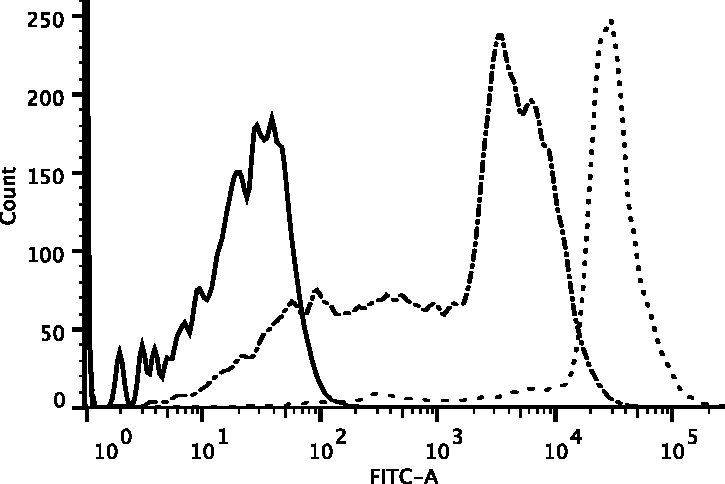
\includegraphics[width=\textwidth]{figs/facs-stable-cell-lines.pdf}
        \captionIntro{Fluorescent intensity of HeLa cell populations
          by flow citometry}%
                     { The multiple populations with differing
                       intensity values were sorted by FACS. The full
                       line represents the intensity profile of HeLa
                       wild type cells, the dash-dot line the mixed
                       population of HeLa cells expressing H2B--EGFP,
                       and the dotted line the homogeneous cell
                       population after sorting.  }
        \label{fig:methods:facs}
      \end{figure}

      Both sample analysis and cell sorting were performed with live cells, the
      first with a BD FACSCanto~II, and the later with a BD FACSAria~II.

  \section{Software used}
    \label{sec:methods:software}
    The European Molecular Biology Open Software Suite (EMBOSS) version 6.4.0
    was used for analysis of codon usage, RNA folding, and reading of
    chromatogram files.

    Image analysis was performed using GNU Octave version \OctaveVersion{},
    and Octave Forge Image, Optim, Statistics, Bioformats, and Signal
    packages, versions \OctaveImageVersion{}, \OctaveOptimVersion{},
    \OctaveStatisticsVersion{}, \OctaveBioformatsVersion{}, and
    \OctaveSignalVersion{} respectively.

    ImageJ, as distributed by the Fiji project, was routinely used
    for microscope image visualization.

  \section{Results}

  \subsection{FRAP analysis in Octave}

  \subsection{Tracking of cell nuclei}

    %% We could show this but it would only be to "encher chouricos"
%    \begin{figure}
%      \centering
%      \missingfigure{Our first FRAP experiment}
%      \captionIntro{Long time series of HeLa cells expressing H2B--EGFP.}
%                   {Cells were transfected with pBOS--H2B-EGFP and imaged for 8
%                    hours, with intervals of 20 minutes.}
%      \label{fig:kill-frap:cell-movement}
%    \end{figure}

    Histone proteins exhibit extremely slow kinetics of exchange
    requiring FRAP to be performed over several hours during which cell movement is
    a particular issue. % \frefp{fig:kill-frap:cell-movement}.

    %% This needs some sentences describing the nature of effects of the movement,
    %% and a semi-emirical statement of the scale of the movement
    %% since this problem is the nub of the entire chapter.
    %% Need to justify the need for going to the trouble
    %% and define threshold for success (that couldn't be achieved!)

    The central requirement to accurately identify and quantitate the signal
    in the photobleached spot led us to pursue both cell biological approaches to
    minimise cell movement and and computational approaches to track imaged regions.

    \subsubsection{Contact inhibition at high cell density}

      Mammalian cells display contact inhibition,
      a cellular growth mechanism by which cells enter senescence and reduce motion
      when surrounded by other cells with no free space for movement.
      Although transformed cell lines lose this property,
      reduced space does place a restriction in the movement.
      %% Can you provide a semi-quantitative estimate of the cell density you mean?
      We attempted to use this effect to limit movement of cells
      by performing FRAP measurements with cells at higher confluence levels.
      We observed some decrease of movement for HeLa cells but not a complete immobilization.
      %% Can you provide a semi-quantitative estimate of the degree of reduction in movement?

      \begin{figure}
        %% We are only showing one cell rather than the whole field of
        %% of view because otherwise it's hard to notice the movement of
        %% individual cells. If we do display everything, we cell many
        %% nuclei that seem like their movement is smaller. If we do
        %% show it, we comment that we are unsure whether the movement
        %% is cellular or only nuclear.
        \centering
        \includegraphics[width=\textwidth]{results/confluent-hela.png}
        \captionIntro{Movement of confluent HeLa cells during FRAP experiment}
          {
            Cells reached confluence before the start of the
            experiment in an attempt to reduce motion. Instead, this caused
            cell nuclei to undergo heavy reshape as the cell apparently
            squeezes in between its neighbours. Half-nuclear FRAP performed in
            a confocal microscope over an interval of 8~hours. Top left panel
            is the pre-bleach image, while the others have a time-interval of
            21~minutes. Cells are a stable line derived from HeLa, expressing
            the H4~R45H mutant tagged with YFP.
          }
        \label{fig:kill-frap:confluent-hela}
      \end{figure}

      Tracking of the ROIs over time was still required \frefp{fig:kill-frap:confluent-hela}.
      %% Isn't this out of order since CropReg section is below.
      %% Even if you did it in a different order, why not put the horse cells first.

    \subsubsection{Primary cell lines}

      Since HeLa cells have lost the ability to activate contact inhibition,
      we obtained an immortalised primary horse fibroblast cell line
      that displayed contact inhibition. Using this cell line we could
      maintain a layer of healthy cells covering a Petri dish for several days???
      after reaching confluence (data not shown).
      %% Cell growth was halted instead of becoming over-confluent ???what do you mean???
      %% Although obvious, it would be good to have some sort of image to justify the statement?

      However, primary cell line transfections have typically much lower efficiency rate and
      confluent cells have lower expression with each cell division.
      To balance transfection efficiency and expression we transfected cells at
      \SI{70}{\percent} confluence and imaged them after 3 days.

      Even after reaching confluence, we observed movement of transfected horse cells \frefp{fig:kill-frap:confluent-horse}.
      %% Is there some sort of relative statement about the degree of reduction or residual movement?
      In addition, the observed movement was dramatically different in primary horse than in HeLa cells.
      Transfected horse cells displayed a helical motion about the vector of their movement
      whereas rotation of HeLa nuclei was mostly restricted to the $z$ axis.
      %% You need to define the coordinate system to talk about z axis!
      %% Do you mean vertical relative to the cell dish layer?

      \begin{figure}
        \centering
        \includegraphics[width=\textwidth]{results/confluent-horse.png}
        \captionIntro{Movement of confluent primary cells during FRAP experiment}
          {
            Primary horse fibrolasts display contact inhibition and halt growth
            once they reach confluence. However, this does not stop cell
            motion which can still be seen moving. In addition, when compared
            to the cancer cell line HeLa \frefp{fig:kill-frap:confluent-hela},
            the horse fibroblasts frequently rotated around the $x$ and $y$
            axis. Circle FRAP was performed in a widefield microscope.
            Top left panel is the pre-bleach image, while the others have a
            time-interval of 15~minutes. Cells were transiently transfected
            and are expressing H2B type1-J tagged with EGFP.
          }
        \label{fig:kill-frap:confluent-horse}
      \end{figure}

    \subsubsection{Tracking of cell movement}

      As an alternative strategy, we implemented cell tracking
      in order to transform images into a common frame using
      consecutive image cropping and image registration.
      This approach was implemented as a program named CropReg.

      Nuclei of interest were tracked by template-based matching using normalized cross-correlation.
      Briefly, the nucleus to track was identified on the first frame and
      used as template against the image on the subsequent frame.
      For increased performance and robustness only the region surrounding the original position is used.
      %% Should you state approximately how large this region was?
      Sequentially applying this method created a stack of smaller images centred on the nuclei of interest.

      Achieving this functionality required implementing a ``coeff'' option
      for scaling in the \texttt{xcorr2} function in GNU Octave.
      This was contributed and released in version 1.2.0 of the Octave Forge signal package.
      %% TODO since there's more than one way to actually do the normalization,
      %% it might be a good idea to write down the actual math formula
      To correct for rotational movement around the $z$ axis,
      frames were aligned using rigid body geometric transformation using ImageJ plugin StackReg \citep{stackreg}.

      \begin{figure}
        \centering
        \includegraphics[width=\textwidth]{results/cropreg.png}
        %% imaging was done every 10 minutes, but we are skipping
        %% every other panel
        \captionIntro{Automatic tracking and alignment of moving cells}
          {
            Using CropReg, we successfully tracked individual cells during
            a time-series microscope experiment. The top left corner of each
            panel displays the tracked and aligned cell. Imaging was performed
            in a widefield microscope. Time interval between panels 20~minutes.
            Cells are a stable line derived from HeLa, expressing H3 tagged
            with YFP.
          }
        \label{fig:kill-frap:cropreg}
      \end{figure}

      Using this image processing approach we were able to track individual cell nuclei
      throughout an entire sequence of FRAP experiments \frefp{fig:kill-frap:cropreg} provided
      that nuclei did not overlap.
      Although only a small minority of image sequences satisfied this requirement,
      it was possible to collect sufficient observations for FRAP calcultions.

  \subsection{Chromatin movement}

    While performing the FRAP experiments, we observed some movement
    within the cell nuclei. These could not be accounted for simple rotational
    movement around the $x$ or $y$ axis, and resembled more the movement
    of individual bodies within the nuclei.

    \subsubsection{Selection of \G1{} cells}
      %% There's no chemical equilibrium in S phase

      A possible cause of this chromatin movement comes from changes in
      the cell cycle phase. During the S~phase, the DNA is replicated,
      doubling the content of the chromatin.
      More importantly, this breaks
      a core assumption of FRAP, that the system remains in equilibrium
      during the entire experiment. This does not hold if the DNA, the
      binding sites for our model, duplicate in number.

      If the FRAP experiments can't be performed during S~phase and
      mitosis, we are limited to \G1{} and \G2{}. Considering
      the length of the HeLa cell cycle and the requirements to image
      for a time period of 8~hours, we are further limited to \G1{}.
      In addition, the FRAP experiment must be performed early in
      \G1{}~phase to avoid crossing over to the S~phase.

      %% The only reason this was required was because the LSM 510
      %% that we were using could not make Z stack and time lapse
      %% at the same time.
%      \begin{figure}
%        \centering
%        \missingfigure{Hela cells splitting}
%        \captionIntro{Picking cells at early G$_1$.}
%                     {We imaged cells that were entering mitosis and picked their
%                      daughter cells for the FRAP experiments. Because HeLa cells lift
%                      away from the dish during mitosis, opening the
%                      pinhole and set the Z-center in between the cell dividing plane
%                      and dish bottom was necessary. Ends up nothing being properly in focus but we
%                      can track things fine. Of course, some cells still floated away.}
%        %% TODO explicit parameters
%        \label{fig:kill-frap:picking-early-g1}
%      \end{figure}

      To do this, cells in mitosis were selected and tracked during 4~hours.
      After this time period, we used the daughter cells which we could be
      confident of being in early \G1{}.
      %% we also waited some 2 hours after mitosis since that's when cells
      %% unpack their chromosomes.

      During mitosis, HeLa cells form a sphere slightly above the plane of
      other cells, and keep a weak connection to the growth surface.
      Because of this, they easily detach, which is the basis for the
      mitotic shake-off method, and float away from the field of vision
      which requires a larger number
      of initial selected cells. In addition, to minimize any effect that
      may arise from imaging, it was done at minimal laser power and every
      30~minutes, just enough to allow manual tracking.
      Finally, since our system did not permit simultaneous Z-stack and time
      lapse imaging, and cells in mitosis are in a separate focal plane,
      imaging was performed with the pinhole sized to the max and focused
      in between the two planes. While this
      created very blurred images, it allowed to visualize all cells during
      the entire procedure.

      However, even after selecting cells in this cell cycle, movement within
      the bleach spot could still be observed.

    \subsubsection{Inverse FRAP}

      Due to the non-homogeneous nature of the chromatin, it was difficult
      to assess the total extent of the observed movement. To
      better visualize this, we performed inverse FRAP which allows us
      to track the movement of the bleach spot only.

      For this purpose, we replaced the EGFP tag in our H2B plasmid
      with photoactivatable GFP (PAGFP), a GFP derivative that requires
      activation by a specific wavelength to become fluorescent. This
      allows us to activate a specific spot of the nucleus and visualize
      its movement.

      Since PAGFP cannot be easily detected before photoactivation, cells
      were co-transfected with mCherry--\textalpha--tubulin which localises
      exclusively to the cytoplasm, giving an outline of the nuclear region
      \frefp{fig:kill-frap:ifrap}.

      \begin{figure}
        \centering
        \subbottom[pre-activation]{
          \includegraphics[width=0.45\textwidth]
          {results/ifrap-pre.png}
          \label{fig:kill-frap:ifrap-pre}
        }
        \hfill
        \subbottom[post-activation]{
          \includegraphics[width=0.45\textwidth]
          {results/ifrap-post.png}
          \label{fig:kill-frap:ifrap-post}
        }
        \subbottom[activated spot over time]{
          \includegraphics[width=\textwidth]
          {results/ifrap.png}
          \label{fig:kill-frap:ifrap-timeframe}
        }
        \captionIntro{Inverse FRAP experiment showing chromatin movement}
          {
            HeLa cells co-transfected with mCherry--\textalpha--tubulin and
            H2B type1-J tagged with PAGFP.
            \subcaptionref{fig:kill-frap:ifrap-pre} The cell nucleus, target
            for photoactivation, can be easily identified as the ``empty''
            region via the mCherry channel on which would otherwise be an
            invisible feature on the GFP channel;
            \subcaptionref{fig:kill-frap:ifrap-post} spot after activation;
            \subcaptionref{fig:kill-frap:ifrap-timeframe} detail of the
            activated spot every 20~minutes. Rather than a gradual loss of
            fluorescence that maintains the circular shape, the activated spot
            kind of unfolds itself spreading the region of interest.
          }
        \label{fig:kill-frap:ifrap}
      \end{figure}

      Using this FRAP variant, the movement of chromatin was more noticeable.
      Rather than an homogeneous loss of fluorescence, the activated
      spot uncurled itself overtime with individual branches of
      localized PAGFP appearing in the nuclei \frefp{fig:kill-frap:ifrap}.

  \section{Discussion}

    We wished to quantitatively determine the
    effect on human chromatin dynamics
    of SIN mutations in core histones H3 and H4 known
    to be destabilising \textit{in vitro} and to affect
    cell growth in \species{S. cerevisiae}.
    We set out to use a previously reported circle FRAP model
    which accounts for multiple factors in a typical
    FRAP modelling \citep{mcnally-frap-code}.

    However, FRAP recovery is incomplete even
    after 8~hours for core histones \citep{KimuraCook}.
    This led us to address a series of technical challenges in
    collecting valid quantitative recovery data over extended time periods.

% Cell movement

    The first problem faced was cell motility, which
    is an expected property of actively dividing cells.
    We attempted to reduce motility by taking advantage of
    the fact that many primary cells display contact inhibition of
    locomotion and proliferation when they reach high densities.
    This contact inhibition is a natural mechanism
    that controls cellular growth in
    multicellular organisms, and results in a stop in proliferation
    with the formation of a monolayer of healthy cells in tissue culture.

    However, the approach has disadvantages including
    increased cell handling and reduced transfection efficiency.
    The potential inability to compare results with published data for
    immortalised cell lines such as HeLa is also undesirable.

    Despite achieving a monolayer of healthy cells that
    could be maintained stably over 2 weeks,
    individual transfected primary horse fibroblasts still showed motility
    despite exhibiting overall characteristics of contact inhibition.
    Furthermore, nuclei in these cells displayed a helical motion
    on the direction of cell movement \frefp{fig:kill-frap:confluent-horse}.

    The possibility of chemically inhibiting
    cells to reduce motion was considered
    since previous FRAP experiments with core
    histones were performed using multiple inhibitors
    of protein synthesis \citep{KimuraCook}. However, these studies revealed
    inhibitor-dependent variations in kinetics and the authors qualified
    their conclusions about the absolute accuracy
    of the histone exchange parameters measured.

    To better address the problem of cell motility we
    instead developed a computational approach
    by writing the program CropReg for cell tracking by normalised
    cross-correlation template matching.
    Using automated analysis enabled us to process
    the large numbers of cell images
    required to provide statistically valid
    quantitative measurements of core histone exchange.

% Compositional changes

    The second challenge to measuring core histone exchange by FRAP is that
    a chemical equilibrium is required between freely diffusing proteins and
    formation of a complex. Although absolute equilibrium is unlikely
    in the dynamic cell environment undergoing
    complex transcriptional and translation responses anyway,
    DNA replication involving polymerase passage
    and repackaging of the duplicated genome
    in S~phase will certainly unbalance any equilibrium.

    Chromosome compaction in mitosis also generates a chromatin environment
    that is distinct from interphase.
    This limits FRAP experiment to either \G1{} or \G2{} phases.
    The HeLa cell cycle has a typical \G1{} phase of 11.7~hours
    and a \G2{} phase of 3~hours \citep{HeLaCellCycle}
    so the extended time periods needed for FRAP of core histones requires
    starting FRAP early in \G1{} \frefp{fig:kill-frap:cell-cycle}.

    Post-mitotic chromosomes take approximately 2~hours
    to migrate within the nucleus
    and rebuild the interphase nuclear architecture during early \G1{}
    \citep{visualizationG1chromosomes,earlyg1position,RelativeChromosomePosition}.
    This defines the window for extended FRAP experiments
    from approximately 3 to 11 hours after mitosis
    in HeLa cells, although cells lines with even longer
    \G1{} phase could also be used \citep{PancreaticCells}.

    We wished to avoid the use of drugs for cell
    cycle arrest since this has been
    shown to influence FRAP results \citep{KimuraCook}.
    We also discounted serum starvation to move cells into the
    quiescent \G0{} phase since this could affect
    the relevance of measuring core histone
    exchange \citep{SerumStarvation}.

      \begin{figure}
        \centering
        %% based on original code from Robert Vollmert
        %% http://www.texample.net/tikz/examples/pie-chart/
        \newcommand{\slice}[4]{
          \pgfmathparse{0.5*#1+0.5*#2}
          \let\midangle\pgfmathresult

          % slice
          \draw[thick,fill=black!10] (0,0) -- (#1:1) arc (#1:#2:1) -- cycle;

          % outer label
          \node[label=\midangle:#4] at (\midangle:1) {};

          % inner label
          \pgfmathparse{min((#2-#1-10)/110*(-0.3),0)}
          \let\temp\pgfmathresult
          \pgfmathparse{max(\temp,-0.5) + 0.8}
          \let\innerpos\pgfmathresult
          \node at (\midangle:\innerpos) {#3};
        }
        \begin{tikzpicture}[scale=3]
          \newcounter{a}
          \newcounter{b}
          %% Total cell cycle is 24.5 hours, G1 is 11.7h, S is 8.8h,
          %% G2 is 3h, M is 1h. The problem is that the counters can't handle
          %% decimal places so we have a variable with the actual time for
          %% the text, and another one times 10 to calculate the angle.
          \foreach \p/\t/\l in {117/11.7/\G1, 9/0.9/M,
                                31/3.1/\G2, 88/8.8/S}
            {
              \setcounter{a}{\value{b}}
              \addtocounter{b}{\p}
              \slice{36*\thea/24.5} % we multiply by 36 instead of 360 because
                    {36*\theb/24.5} % the time is already times 10
                    {\l}{\t{} hours}
            }
        \end{tikzpicture}
        \captionIntro{HeLa cell cycle phases and timing}
          {
            Under optimal growth conditions the HeLa cell has a median
            doubling time of 24~hours, with \G1~and
            S~phases of 11.7 and 8.8 hours respectively \citep{HeLaCellCycle}.
          }
        \label{fig:kill-frap:cell-cycle}
      \end{figure}

    Instead, we developed a procedure to track
    progression of cells manually during mitosis
    where visual identification of the cell cycle is possible.
    This allowed us to minimise the variations of normal cell growth
    and to identify individual cells exactly 3 hours after start of \G1{}.
    This has the added advantage of allowing time for maturation of GFP
    expressed during the establishment of interphase.
    The time interval between images during manual selection was increased and
    both resolution and laser intensity were reduced
    to minimise phototoxicity or bleaching.
    This resulted in a set of selected early \G1{}
    cells suitable for FRAP experiments.

    The fluorescently tagged histone proteins are constitutively expressed
    under the control of an EF-1\textalpha{} promoter,
    so they lack the 3' regulatory features of native histone genes.
    This regulation does not follow the normal
    expression program of a histone gene
    and could affect the distribution of the histone in chromatin.
    Constant expression of tagged histones by a strong constitutive promoter
    will enrich them in the \G1{} and early S~phase pools
    making subsequent incorporation in euchromatin more likely,
    relative to mid-late S~phase where heterochromatic sequences
    are replicated and packaged \citep{DNA-replication-timing}.

    A more realistic tagged histone expression profile could be achieved using
    flanking regulatory regions from native histone genes,
    as demonstrated for H3 and CENP--A \citep{pMH3-plasmid,Kevin-pCA-TAG}.
    Another potential solution is to insert GFP
    in-frame into the native gene locus by genome engineering,
    although the redundancy between the multiple canonical histone genes means
    that identifying the most appropriate isoform to target
    could introduce complexities.

    Protein synthesis inhibitors were used by \citet{KimuraCook}
    to address this issue,
    but this has the disadvantage of potentially affecting
    many other processes as discussed above.

      %% TODO: would be cool to create this figure
%      \begin{figure}
%        \centering
%        \missingfigure{a schematic of cell cycle, soluble pool}
%        \captionIntro{Distribution of tagged and endogenous histones during cell cycle}
%                     {
%                       This would be at least 3 different subplots. The first
%                       and the second are like the ones in Fig 7A of Kimura and
%                       Cook paper. The third one would show the ratio of each
%                       histone over time, i.e., 100\% tagged during all cell
%                       cell cycle and some endogenous during S phase. In this
%                       plots, also note where euchromatin and heterochromatin
%                       are replicated.
%                     }.
%        \label{fig:kill-frap:messy-histone-expression}
%      \end{figure}

% Movement of the reference

    The final challenge to measuring core histone
    exchange by FRAP that we identified
    was non-homogenous regional movement of chromatin itself.

    One possible cause for this movement is chromatin repackaging
    during DNA replication which we addressed by selecting cells at
    early \G1{} phase.
    One other cause is chromatin remodelling as part of a DNA damage
    response caused by the FRAP photobleaching event itself.
    The phototoxicity effects of a FRAP experiment are often dismissed
    on the basis that the photobleaching event of a typical FRAP
    experiment does not affect cell viability
    \citep{kruhlak2000reduced, KimuraCook, carrero2003using} but the
    DNA damage that such experiment may introduce, and the effect that
    the repair response of such damage may have on chromatin
    reconfiguration, has not yet been addressed.
    Still, the use of laser beams of different wavelength and longer
    exposure times are often used to introduce both single and double
    DNA strand breaks on which FRAP experiments are then performed
    \citep{stixova2014advanced, mari2006dynamic, kim2002specific}.

    Independently of the cause for the chromatin movement,
    it undermines the assumption of FRAP analysis that binding sites
    remain immobile throughout the FRAP experiment.
    This assumption is required to interpret recovery
    as the rate of movement of freely diffusing unbleached molecules into the
    bleached area which allows the kinetic
    rates \kon{} and \koff{} to be estimated.
    If chromatin binding sites also move then the recovery curve becomes a
    much more complex function of both binding site movement and free diffusion.

    Chromatin movement is recognisable
    by changes in the intra-nuclear features of the fluorescent chromatin
    and by changes in the circular bleach spot.
    Although some of these effects are subtle when observed by photobleaching,
    the photoactivation of an equal circular spot demonstrates
    clear non-homogenous reshaping of chromatin.
    Equivalent chromatin movement has also been reported
    for H4--PAGFP in strip photoactivation \cite{H4PAGFP-chromatin-movement}.

    The movements we observed were in the
    range of \SI{4}{\um}, which is double the size of the bleach spot,
    and exhibited complicated shapes reminiscent of channelling.
    This is consistent with chromosome distribution in nuclei that is
    territorial on the scale of \SI{5}{\um} \citep{sun2000size}
    separated by interchromosomal channels of
    \SIrange{10}{100}{\nm} \citep{gorisch2005histone}.

    The clarity of H2B--GFP imaging by photoactivation
    suggests the opportunity to analyse the
    paths taken by diffusing core histones.
    For example, simultaneous use of combined
    photoactivation and photobleaching
    of complementary dimer and tetramer histones could
    enable relative diffusion rates and paths to be determined.
    Alternatively, an enzymatic mechanism to incorporate a
    complementary photo-differented label
    into DNA  would facilitate masking for
    the original location at the same time as tracking the histone diffusion
    and enable quantitative FRAP.
    Nevertheless, it is important to recognise
    that such experiments would test the
    resolution and sensitivity of microscopes.

\section{Conclusion}

    Since its inception over 30 years ago, FRAP has been continuously
    improved
    through technical capabilities of light microscopy
    and sensitive kinetic models that are now able to take into account
    an increasing number of biophysical features such as container size,
    non-homogeneous distribution of fluorescence, and profile of bleach spot.

    Despite these advances, the ability to perform FRAP
    over extended time periods of several hours for highly stable complexes
    such as core histones is limited by the dynamic nature of the cell.

    We overcame the challenges of cell motility
    and selection of cells in \G1{} phase,
    but were not able to develop a method to adjust
    for changes in chromatin structure within the cell nucleus.
    While a photobleached spot appears stable and
    can be tracked over several hours,
    small natural disturbances and non-homogeneous diffusion
    impact on photorecovery
    and estimation of kinetic parameters.
    We find that FRAP is suitable for semi-quantitative
    estimates of slowly diffusing molecules
    but not for the precise quantitative comparisons
    required to compare core histone mutations.

    Ultimately, the issue of long observation times stems from the
    requirements of FRAP models to achieve full recovery of the mobile
    populations being measured.

    Single particle tracking is a microscopy technique where, as the
    name suggests, the motion of isolated molecules is observed.  In
    this technique, a small number of particles, small enough that
    they can be resolved and their individual movements tracked, is
    observed over a short amount of time, typically on the scale of
    seconds.  The short time is a limitation and not a requirement of
    the technique, and is caused by observational photobleaching.
    This would remove the requirement of hours long observation and
    overcome the issue of chromatin movement.  In addition, it would
    provide an overview of different types of protein motion where
    FRAP would only provide an average of the movement, and as a super
    resolution microscopy technique, would also be able to identify
    confined movement that FRAP would otherwise classify as immobile
    as been previously the case of MHC class I proteins
    \citep{smith1999anomalous}.
    However, the high concentration of histones in the nucleus makes
    it challenging to observe the required individual molecules.  This
    could possibly be overcame with the use of photo-activatable FPs
    such as PAGPF which would allow for the activation of a small
    population and the use of a Selective Plane Illumination
    Microscopy (SPIM) which allows the observation and excitation of
    fluorescent molecules in a single focal plane.

    Fluorescence Correlation Spectroscopy (FCS) is a fluorescent
    microscopy technique providing estimates of dynamic parameters by
    using fluorescence fluctuations in a femtolitre volume.
    More spatiotemporal dynamics can be obtained by observing the
    fluorescence fluctuations while moving the measurement volume
    across the sample, a technique named Spatio-Temporal Image
    Correlation Spectroscopy (STICS) \citep{hebert2005spatiotemporal}.
    One other variation of FCS is Raster Scan Image Correlation
    Spectroscopy (RICS) which is similar to STICS but can be performed
    on a standard confocal microscope \citep{digman2005rics}.  In both
    cases, image regions that may span the entire cell nuclei may be
    observed and populations with different dynamics localised within
    it.  Such techniques
    could potentially provide not only a method to compare core
    histone mutations \textit{in vivo} but also their effect in
    different chromatin domains.
    However, their implementation is still difficult, from the
    optimisation of scanning parameters to the complex data
    processing, and there are not many papers on the literature
    reporting their use outside the laboratory that developed them.

    Overall, the current period of rapid technological advances in
    cell biology research means that new techniques such as RICS and
    single particle tracking offer
    hope to address specific challenges such as histone mobility for
    which existing approaches such as FRAP are poorly suited.

%  Single-molecule imaging of histones for short period of times in
%  live cells has recently been reported using super-resolution
%  imaging\addref[nature methods 7(9):717-719, 2010 and nature methods
%  8(1):7-9, 2011].

%  Also, use of PAGFP has been used to measure dynamics of H4 over
%  \SI{90}{\ms} reporting differences between interphase chromatin and
%  mitotic chromosomes\addref[Saera Hihara et al 2012].  However, the
%  difference between these two phases is the highest and might not be
%  comparable to the difference between histones variants\todo{study
%  this. Someone must have measured this}.


  \chapter{Dynamics of CENP HFD}
\label{ch:cenp}

%% if at first you don't succeed, run -- a softer world

\section{The FRAP/FLAP model}
\section{Development of MaryI}
\section{HFD association rates}
\section{HFD stoichiometry on the kinetochore}
\section{Involvement of FACT in assembly of CENP–T/W complex}
\section{Cell cycle}
  \subsection{Timing of assembly with respect to DNA replication}
  \subsection{Dynamics as a function of the cell cycle phase}
\section{Requirements for CCAN in HFD CENP assembly}
  \subsection{CENP–T/W influence on CENP–S/X}
\section{Conclusions}

  \subinputfrom{software/}{software}

  \chapter{Conclusion}
\label{ch:conclusion}

  %% \epigraph{tl;dr}{}
  %% \epigraph{when the going gets tough, the tough get cardboard sleeves because the
  %%           cups too hot.}{Doghouse diaries #5051}

  \appendix
\chapter{Solutions}
  \label{app:solutions}
  
  %% an alternative method to make this lists is with description environment
  %%
  %% \begin{description}
  %%   \item[Freezing media] \hfill \\
  %%     91\% FCS;
  %%     10\% DMSO
  %%   \item[Growth medium (HeLa)] \hfill \\
  %%     87\% DMEM;
  %%     10\% FCS;
  %%     1\% NEAA;
  %%     ...
  %% \end{description}
  
  %% This requires the eqparbox package. It checks what LaTeX thinks is best for a column
  %% and save that value. It will then use it to calculate what's left of \textwidth, and
  %% use it for the other columns. See http://tex.stackexchange.com/questions/95397
  %% It doesn't work with memoir's ctabular so we are using longtable instead
  \newsavebox{\firstentrybox}
  \newcolumntype{N}{%
    >{\begin{lrbox}{\firstentrybox}}%
      l%
    <{\end{lrbox}%
    \eqmakebox[firstentry][l]{\unhcopy\firstentrybox}}}

  \begin{longtable}{>{\bfseries}N p{\dimexpr(\textwidth-\eqboxwidth{firstentry}-4\tabcolsep)}}
    \toprule
    Name & Recipe\\
    \midrule
    2YT broth               & \\
    %% FIXME get 2YT media recipe
    
    DMEM                    & \SI{4.5}{\g\per\l}   glucose;
                              \SI{110}{\mg\per\l}  L-glutamine;
                              \SI{584}{\ug\per\l}  sodium pyruvate;
                              \SI{15.9}{\mg\per\l} phenol red.\\
    
    DNA loading buffer (10$\times$) & \pcent{25} Ficoll ($w/v$);
                              \SI{100}{\mM}      Tris--HCl pH=\num{7.4};
                              \SI{100}{\mM}      EDTA.\\
    
    Freezing media          & \pcent{90} FCS;
                              \pcent{10} DMSO.\\
    
    Growth medium (HeLa)    & \pcent{89}            DMEM;           % 500ml
                              \pcent{9}             FCS;            % 50ml
                              \SI{1}{$\times$}      NEAA solution;  % 5.5mL
                              \SI{50}{units\per\ml} penicillin;     % 5.5mL (Pen/Strep solution)
                              \SI{50}{\ug\per\ml}   streptomycin.\\ % 5.5mL (Pen/Strep solution)
    
    Growth medium (horse)   & \pcent{81}            DMEM;           % 500ml
                              \pcent{16}            FCS;            % 100ml
                              \SI{2}{$\times$}      NEAA solution;  %  12mL
                              \SI{50}{units\per\ml} penicillin;     % 5.5mL (Pen/Strep solution)
                              \SI{50}{\ug\per\ml}   streptomycin.\\ % 5.5mL (Pen/Strep solution)
    
    %% TODO check exactly the LB recipes
    LB agar                 & \pcent{2}   LB ($w/v$);
                              \pcent{1.5} agar.\\
    
    LB broth                & \pcent{2} LB ($w/v$).\\
    
    PBS                     & \\
    %% TODO check exact PBS recipe from the tablets
    
    Ponceau S solution      & \pcent{5} Ponceau-S ($w/v$);
                              \pcent{5} Acetic acid ($v/v$).\\
    
    Running buffer          & \SI{1}{$\times$} TG;
                              \pcent{0.1}      SDS ($w/v$).\\
    
    SSC (Saline Sodim Citrate) & \SI{150}{\mM} NaCl;
                              \SI{15}{\mM}     Trisodium citrate.\\
    
    TAE (Tris Acetate EDTA) & \\
    %% TODO get TAE buffer recipe
    
    TBE (Tris Borate EDTA)  & \SI{89}{\mM} Tris;
                              \SI{89}{\mM} Boric acid;
                              \SI{2}{\mM}  EDTA.\\
    
    TBS (Tris Buffered Saline)  & \SI{50}{\mM} Tris--HCl pH=\num{7.5};
                              \SI{100}{\mM}    NaCl.\\
    
    PBS-T (TBS-Tween)       & \pcent{99.95} PBS ($v/v$);
                              \pcent{0.05}  Tween 20 ($v/v$).\\
    
    TG (Tris Glycine)       & \SI{25}{\mM}  Tris;
                              \SI{192}{\mM} glycine.\\
    
    Transfer buffer         & \SI{1}{$\times$} TG;
                              \pcent{15} methanol ($v/v$).\\
    \bottomrule
  \end{longtable}
    

\chapter{List of plasmids}
  \label{app:plasmids}
  %% generate this automatically from SQlite db
  %% should we print the maps on genbank format, just the genbank features
  %% table, or a draw of the map, poiting to the database for the sequence
  %% details?

\chapter{List of primers}
  \label{app:primers}
  %% generate this automatically from SQlite db


  \backmatter

  \bibliography{%
    intro/references,%
    methods/references,%
    software/references,%
    histone-catalogue/references,%
    kill-frap/references,%
    fancy-frap/references,%
    h2ax-review/H2AXreview-biblio%
  }

\end{document}
